% ============================================================
% main.tex — Master Thesis
% Title: CoG-Based Geometric Constraints and Custom Fingertip
%         Design for Reliable Industrial Deployment of
%         vMF-Contact Grasping on a UR10e Collaborative Robot
% Author: Yimin Hu
% Affiliation: Karlsruhe Institute of Technology (KIT)
%              SFB-1574 Circular Factory
% Date: 2026
% Citation style: IEEE
% ============================================================
% PENDING BEFORE SUBMISSION:
%   [X] Fill Tables 4.1, 4.2, 4.3 from experimental logs
%   [X] Substitute exact chi-squared statistics in Section 4.2.1
%   [ ] Verify 72.7% figure against ICRA 2025 proceedings PDF
%   [X] Enter total end-to-end cycle time in Section 3.6
%   [ ] Verify full author lists: cai2024, shi2025
%   [ ] Insert Figures 3.1, 3.2, 3.3
%   [X] Add abstract (use /ars-abstract)
%   [X] Add AI-usage disclosure statement (use /ars-disclosure)
% ============================================================

\documentclass[12pt, a4paper]{report}

% --- Page layout ---
\usepackage[a4paper, top=2.5cm, bottom=2.5cm, left=3cm, right=2.5cm]{geometry}

% --- Typography ---
\usepackage{microtype}
\usepackage{setspace}
\onehalfspacing
\setlength{\parindent}{0pt}
\setlength{\parskip}{8pt}

% --- Mathematics ---
\usepackage{amsmath, amssymb}

% --- Graphics and tables ---
\usepackage{graphicx}
\usepackage{booktabs}
\usepackage{caption}
\usepackage{array}
\usepackage{multirow}
\usepackage[table]{xcolor}
\graphicspath{{images/}}

% --- Bibliography (IEEE style) ---
\usepackage{cite}

% --- Headers and footers ---
\usepackage{fancyhdr}
\pagestyle{fancy}
\fancyhf{}
\fancyhead[L]{\nouppercase{\leftmark}}
\fancyhead[R]{\thepage}
\renewcommand{\headrulewidth}{0.4pt}
\fancypagestyle{plain}{
  \fancyhf{}
  \fancyfoot[C]{\thepage}
  \renewcommand{\headrulewidth}{0pt}
}

% --- Hyperlinks ---
\usepackage[hidelinks, breaklinks=true]{hyperref}
\usepackage{url}
\usepackage{cleveref}

% --- Code/parameter names ---
\newcommand{\param}[1]{\texttt{#1}}

% --- Placeholder boxes for figures ---
\newcommand{\figplaceholder}[2]{%
  \begin{figure}[htbp]
    \centering
    \fbox{\parbox{0.7\textwidth}{\centering\vspace{2cm}%
      \textit{[Figure placeholder: #1]}\vspace{2cm}}}
    \caption{#2}
  \end{figure}%
}

% ============================================================
\begin{document}

% ============================================================
% TITLE PAGE
% ============================================================
\begin{titlepage}
  \centering
  \vspace*{2cm}

  {\LARGE\bfseries
    CoG-Based Geometric Constraints and Custom Fingertip Design\\[0.4em]
    for Reliable Industrial Deployment of vMF-Contact Grasping\\[0.4em]
    on a UR10e Collaborative Robot\par}

  \vspace{1.5cm}
  {\large Master's Thesis\par}
  \vspace{0.5cm}
  {\large submitted in partial fulfilment of the requirements\\
    for the degree of Master of Science\par}

  \vspace{2cm}
  {\large by\par}
  \vspace{0.5cm}
  {\Large\bfseries Yimin Hu\par}

  \vspace{2cm}
  {\large
    Karlsruhe Institute of Technology (KIT)\\
    SFB-1574 Circular Factory for the Future\\
    \par}

  \vfill
  {\large June 2026\par}
\end{titlepage}

% ============================================================
% FRONT MATTER
% ============================================================
\pagenumbering{roman}

\chapter*{Abstract}
\addcontentsline{toc}{chapter}{Abstract}

\section*{English}

Learning-based grasp generation methods achieve strong benchmark performance but consistently fall short in real industrial deployment. This thesis addresses two systematic limitations of the vMF-Contact algorithm on a UR10e collaborative robot. The robot handles an angle grinder in a circular manufacturing cell. Candidate generation lacks object-level geometric priors, and deployment evaluation lacks a structured methodology.

Two algorithmic and one hardware contribution are presented. Centroid-based geometric constraints enter the vMF-Contact pipeline as a post-inference filter. An annular grip-zone bound, relative to the object's geometric centroid proxy, corrects grip force insufficiency. A gripper-axis alignment constraint eliminates placement orientation errors. A custom fingertip replaces the stock Robotiq 2F-140 tip. Its curved contact profile matches the angle grinder's cylindrical handle. A silicone friction layer addresses residual grip failures that persist after algorithmic correction. Both adaptations are integrated in a reproducible ROS2 and Docker deployment pipeline.

A factorial evaluation across 432 trials tested three conditions. These were an unconstrained baseline, the constrained algorithm, and the constrained algorithm with custom fingertip. This design isolates the contribution of each adaptation. Unconstrained vMF-Contact achieves 13.9\,\% success; centroid-based constraints raise this to 40.3\,\%; the custom fingertip raises it further to 77.1\,\%. The 77.1\,\% result exceeds the published vMF-Contact benchmark of 72.7\,\%. This holds despite three compounding deployment disadvantages: 47\,\% lower grip force, twice the object weight, and a stricter pick-transport-place criterion. Failure mode analysis identifies constraint-induced kinematic infeasibility as the dominant residual failure mechanism.

\vspace{0.5cm}
\noindent\textbf{Keywords:} robotic grasping, vMF-Contact, centroid-based constraints, industrial deployment, pick-and-place, collaborative robot, uncertainty-aware grasping

\vspace{1cm}
\section*{Zusammenfassung (Deutsch)}

Lernbasierte Greifgenerierungsmethoden erzielen in Benchmark-Evaluierungen hohe Erfolgsraten, scheitern jedoch regelmäßig beim Einsatz in realen industriellen Umgebungen. Diese Arbeit identifiziert und adressiert zwei systematische Einschränkungen des vMF-Contact-Algorithmus beim Betrieb auf einem kollaborativen UR10e-Roboter für die Handhabung einer Winkelschleifmaschine in einer Kreislauffertigungszelle: das Fehlen objektbezogener geometrischer Vorannahmen bei der Kandidatengenerierung sowie das Fehlen einer strukturierten Methodik zur Bewertung realer Deployments.

Es werden zwei algorithmische und ein hardwareseitiger Beitrag vorgestellt. Schwerpunktbasierte geometrische Einschränkungen werden als Post-Inferenz-Filter in die vMF-Contact-Pipeline integriert: Eine ringförmige Greifzonengrenze relativ zum geometrischen Schwerpunkt-Proxywert des Objekts behebt Greifkraftmangel, während eine Greifer-Achsenausrichtungsbeschränkung Orientierungsfehler bei der Ablage eliminiert. Ein maßgefertigter Ersatz-Fingertip für den Robotiq 2F-140, mit einem an das zylindrische Handgriffprofil der Winkelschleifmaschine angepassten Kontaktprofil und einer Silikonreibungsschicht, behebt die nach der algorithmischen Korrektur verbleibenden Greiffehler. Beide Anpassungen sind in einer reproduzierbaren ROS2- und Docker-Deployment-Pipeline integriert.

Eine faktorielle Evaluation über 432 Versuche unter drei Bedingungen isoliert den Beitrag jeder Anpassung: Uneingeschränktes vMF-Contact erreicht eine Erfolgsrate von 13,9\,\%; schwerpunktbasierte Beschränkungen steigern diese auf 40,3\,\%; der maßgefertigte Fingertip erhöht sie weiter auf 77,1\,\%. Dieses Ergebnis übertrifft den publizierten vMF-Contact-Benchmark von 72,7\,\% trotz drei erschwerender Deploymentbedingungen: 47\,\% geringere Greifkraft, doppeltes Objektgewicht und ein strengeres Erfolgskriterium für den vollständigen Greif-Transport-Ablage-Vorgang. Die Fehlermodusanalyse identifiziert constraint-induzierte kinematische Unerreichbarkeit als dominanten verbleibenden Fehlermechanismus.

\vspace{0.5cm}
\noindent\textbf{Schlüsselwörter:} Robotergreifen, vMF-Contact, schwerpunktbasierte Beschränkungen, industrielles Deployment, Pick-and-Place, kollaborativer Roboter, unsicherheitsbewusstes Greifen

\chapter*{Acknowledgements}
\addcontentsline{toc}{chapter}{Acknowledgements}
This work was supported by the Deutsche Forschungsgemeinschaft (DFG) under the project SFB-1574 ``Circular Factory for the Future.'' The author thanks the Circular Factory Working Group C for access to the CT-cell infrastructure and the UR10e deployment cell.

\chapter*{Declaration}
\addcontentsline{toc}{chapter}{Declaration}
I hereby declare that this thesis is my own original work and that I have not used any sources or aids other than those indicated. All passages taken verbatim or in paraphrase from published or unpublished works have been duly attributed.

\vspace{1.5cm}
\noindent Karlsruhe, \hspace{3cm} \underline{\hspace{5cm}}\\
\hspace*{4.5cm} Yimin Hu

\chapter*{AI-Usage Disclosure}
\addcontentsline{toc}{chapter}{AI-Usage Disclosure}

This thesis was prepared with the assistance of large language model (LLM) tools. The following AI system was used:

\begin{itemize}
  \item \textbf{Claude Code (Anthropic):} Used for academic writing assistance, including prose editing and refinement, structural feedback on chapter organisation, simulated peer-review commentary for revision guidance, bilingual abstract generation (English and German), and numerical consistency checking across chapters. All AI-assisted text was reviewed against experimental data and either accepted, revised, or rejected by the author before inclusion.
\end{itemize}

The following components were performed exclusively by the author without AI assistance: experimental design, hardware fabrication and characterisation, all 432 robot trials and data collection, quantitative data analysis, and the intellectual contributions described in Sections~1.3 and 6.2. The research questions, hypotheses, experimental results, failure mode classifications, and conclusions are the author's own.

This disclosure is made in accordance with the guidelines of the Karlsruhe Institute of Technology (KIT) on the use of AI tools in academic work (academic year 2025--2026). The author accepts full responsibility for the accuracy, integrity, and originality of all content in this thesis.

\tableofcontents
\listoffigures
\listoftables

% ============================================================
% MAIN MATTER
% ============================================================
\pagenumbering{arabic}

% ============================================================
\chapter{Introduction}
% ============================================================

\section{Motivation}
\label{sec:motivation}

In circular manufacturing, returned products arrive with variable geometry, orientation, and positional offset. For a pick-and-place robot operating in this environment, a grasp program calibrated to a single nominal pose fails the moment the object deviates from the assumed configuration --- a deviation that occurs, by design, on every return cycle. The automated guided vehicles (AGVs) that deliver components to the cell operate with positioning tolerances of $\pm$30\,mm or more; the same angle grinder may arrive at a different orientation and position on each inspection pass. Flexible grasping is therefore not an enhancement to the existing workflow. It is a structural requirement of the circular factory paradigm.

\section{Background}
\label{sec:background}

\subsection{The Circular Factory}
\label{sec:background-circular-factory}

The work in this thesis is conducted within the SFB-1574 Circular Factory for the Future, a research programme funded by the Deutsche Forschungsgemeinschaft (DFG, project number 471687386) at the Karlsruhe Institute of Technology (KIT). The programme develops manufacturing systems in which linear production and circular recovery operations --- remanufacturing, refurbishment, and material recycling --- are integrated within a single, flexible production environment~\cite{lanza2024vision}.

A circular factory is characterised by modular and adaptable production hardware that can be reconfigured as process demands change~\cite{bail2025circular}. It consists of three types of stations: \textit{production stations} that carry out remanufacturing processes, \textit{inspection stations} that assess product quality and condition, and an \textit{adaptive intralogistics system} that provides flexible material flow between them. The intralogistics system is realised by a fleet of mobile manipulators equipped with heterogeneous functional modules. Three module types serve distinct roles: buffer modules provide mobile intermediate storage, transport modules convey products between locations, and \textit{manipulator modules} perform the physical handling of products at the interface between the intralogistics system and the production stations~\cite{bail2025circular}.

The manipulator module comprises a robotic arm equipped with camera sensors for product recognition and the capability to execute object-centric grasp plans. Bail et al.~\cite{bail2025circular} specify that grasp planning in the manipulator module relies on an intelligent grasp planner with uncertainty quantification, citing the vMF-Contact algorithm~\cite{shi2025} as the intended planning component. Returned products arrive at the cell via automated guided vehicles (AGVs) that operate with positioning tolerances of $\pm$30\,mm or more, meaning the object's position and orientation at delivery are not known in advance. The manipulator module must therefore execute reliable pick-and-place operations over the full range of possible delivery configurations, making flexible grasping a structural requirement rather than an optional enhancement.

\subsection{The Deployment Cell and Target Object}
\label{sec:background-deployment-cell}

The robot station evaluated in this thesis constitutes a manipulator module deployed within the intralogistics system of the SFB-1574 cell. Its specific function is to receive angle grinders delivered by AGVs, execute a pick-and-place operation that transfers each grinder to the CT scanner placement zone for inspection, and return to the home position. This is one of the core intralogistics operations in the circular factory: adaptive manipulation and transfer of end-of-life products between stations under positional and geometric uncertainty.

The station consists of a UR10e 6-axis collaborative robot arm (Universal Robots, Odense, Denmark), an Orbbec Femto Mega RGBD camera for depth-based point-cloud perception, and a Robotiq 2F-140 parallel-jaw gripper. The angle grinder selected as the target object is representative of the product class handled in the cell: it has an elongated, asymmetric geometry with a cylindrical handle. Its handle cross-section requires a jaw opening exceeding 85\,mm to achieve full gripper closure, necessitating the Robotiq 2F-140 (140\,mm maximum jaw opening, 125\,N maximum grip force) rather than the Robotiq 2F-85 (85\,mm, 235\,N). This geometric compatibility requirement imposes a 47\,\% reduction in maximum grip force relative to the 2F-85 --- a hardware constraint with direct consequences for grasp reliability that is examined throughout this thesis.

\subsection{The vMF-Contact Grasping Algorithm}
\label{sec:background-vmf-contact}

The vMF-Contact algorithm~\cite{shi2025} serves as the grasp generation component of the manipulator module pipeline. Given a point cloud of the target object, it produces a ranked set of 6-DoF grasp candidates. Rather than assigning a single quality score to each candidate, the method models the distribution of contact normals using von Mises-Fisher (vMF) distributions --- a probability distribution over the unit hypersphere suited to directional data --- and generates candidates by sampling from this distribution weighted by estimated probability mass.

This formulation captures two qualitatively different sources of prediction uncertainty. Aleatoric uncertainty arises from sensor noise, reflective surfaces, and occlusion; it is irreducible regardless of training data volume because it is a property of the physical sensing environment. Epistemic uncertainty arises from the model's limited exposure to certain object geometries or viewpoints; it is reducible in principle with additional training coverage~\cite{kendall2017uncertainties}. The operational significance of epistemic uncertainty is that it provides a detectable signal when the model is extrapolating beyond its training distribution --- a property that proves consequential in the evaluation reported in Chapter~4.

Shi et al.~\cite{shi2025} report a benchmark success rate of 72.7\,\% for vMF-Contact on diverse objects evaluated on a Robotiq 2F-85 gripper platform. The benchmark metric is isolated grasp detection --- whether the gripper achieves stable closure --- and does not include object transport, placement accuracy, or downstream task success. The gap between this 72.7\,\% benchmark result and the performance observed in the SFB-1574 deployment cell, and the structural reasons for that gap, motivate the research questions and contributions of this thesis.

\section{Research Questions}
\label{sec:research-questions}

The primary research question is: to what extent can the pick-and-place with unconstrained vMF-Contact algorithm work in a real production scenario? What other constraints can be applied to improve the grasping success rate and placement orientation consistency of an angle grinder compared to unconstrained vMF-Contact inference?

A secondary question examines failure distribution: under which object orientations and positions does the constrained method fail, and through which failure mode?

\section{Contributions}
\label{sec:contributions}

This thesis makes four contributions.

\textbf{Contribution A --- Centroid-based geometric constraints.} Two parameter-governed constraints are introduced into the vMF-Contact inference pipeline: a gripper zone bound relative to the object's geometric centroid proxy, controlling the annular region within which grasp candidates are accepted, and a gripper-axis alignment constraint with the object's longest principal axis. Together, these confine candidates to positions that are mechanically sufficient and orientationally consistent with the downstream task.

\textbf{Contribution B --- Custom fingertip design.} A replacement fingertip for the Robotiq 2F-140 gripper is designed and fabricated, incorporating a curved contact profile matched to the angle grinder handle cross-section and a silicone friction layer. The design targets grip force insufficiency, the dominant failure mode under the constrained algorithm with the original fingertip. Contribution B is a hardware engineering adaptation to the specific hardware-object pairing of this deployment, distinct from the algorithmic extension of Contribution A. Both adaptations are necessary; their independent necessity is examined by the three-condition factorial experiment as introduced in \cref{sec:experimental-overview}.

\textbf{Contribution C --- ROS2 and Docker integration pipeline.} The constrained algorithm is integrated into a reproducible ROS2 pipeline with Docker containerisation, enabling deployment on the UR10e, Orbbec Femto Mega depth camera, and Robotiq 2F-140 gripper cell with minimal environment configuration.

\textbf{Contribution D --- Structured deployment evaluation.} A factorial evaluation across 432 trials under three conditions --- unconstrained baseline~1 , constrained baseline~2, and final conditon with constrained algorithm and custom fingertip--- isolates the contribution of each adaptation. The evaluation stratifies failure modes by object orientation and position, identifies residual failure clusters, and provides a specific remediation path for each failure type.

\section{Experimental Overview and Key Results}
\label{sec:experimental-overview}

Evaluation is conducted across 144 trials structured as a 6-position $\times$ 8-orientation $\times$ 3-repetition matrix under three conditions. Baseline~1 runs unconstrained vMF-Contact inference with the original Robotiq fingertip. Baseline~2 runs the centroid-constrained algorithm with the same fingertip. The Final condition uses the centroid-constrained algorithm with the custom fingertip. This factorial design isolates the software contribution (Baseline~1 versus Baseline~2) from the hardware contribution (Baseline~2 versus Final).

Baseline~1 achieves a success rate of 13.9\,\%, confirming that unconstrained inference is not viable for the task. Baseline~2 reaches 40.3\,\%, demonstrating that centroid-based constraints produce a substantial and necessary improvement. The Final condition achieves 77.1\,\%, demonstrating viability under conditions more demanding than the published vMF-Contact benchmark of 72.7\,\%~\cite{shi2025} which encompassed the full pick-transport-place sequence with lower grip force, a heavier object, and a stricter success criterion. 

Learning-based grasping methods achieve strong benchmark performance. However, industrial deployment consistently falls short of these results. The central question this thesis addresses is how to close this gap.

\section{Thesis Structure}
\label{thesis-structure}

Chapter~2 traces the development of robotic grasping from model-based registration to uncertainty-aware deep learning, establishing the research gaps this work addresses. Chapter~3 describes the system design and methodology: hardware configuration, centroid-based constraint formulation, fingertip design, and the ROS2 integration pipeline. Chapter~4 presents the experimental protocol, trial matrix, results across all three conditions, and a failure mode analysis. Chapter~5 discusses the implications of these results for algorithm design, hardware selection, and industrial deployment practice. Chapter~6 concludes and identifies directions for future work.


% ============================================================
\chapter{Related Work}
\label{chap:related-work}
% ============================================================

\section{Model-Based Grasping}
\label{sec:model-based-grasping}

The theoretical foundations of robotic grasping rest on contact mechanics and force-closure analysis. Bicchi and Kumar~\cite{bicchi2000robotic} established the analytical framework for characterising grasp stability through contact force models, friction constraints, and kinematic conditions for force closure --- principles that remain the basis for both model-based and, indirectly, learning-based grasp evaluation. Parallel-jaw grippers operating on rigid objects, as used in this thesis, represent the most widely deployed instantiation of these principles in industrial practice.

Operationally, model-based systems couple pose estimation with a pre-programmed grasp. Given a CAD model and a point cloud from a depth sensor, ICP~\cite{besl1992} estimates the rigid transformation that aligns the scan to the stored model, recovering object pose. A robot program then applies the corresponding grasp. Rusu et al.~\cite{rusu2009fast} extended the registration toolkit with Fast Point Feature Histograms (FPFH), which encode local surface curvature into compact feature vectors and enable faster convergence than nearest-point search alone, as well as better initialisation for ICP in the presence of partial occlusion. The Point Cloud Library (PCL)~\cite{rusu2011pcl} consolidated these and other point-cloud algorithms into a widely used open-source framework that underpins most depth-sensor-based robotic perception pipelines.

Physics-based simulation environments such as GraspIt!~\cite{miller2004graspit} made it possible to enumerate and evaluate grasp configurations analytically before deployment, accelerating the development of model-based systems and generating the annotated grasp databases that later informed data-driven approaches. Bohg et al.~\cite{bohg2014data} survey the landscape of data-driven grasp synthesis across both model-based and early learning-based methods, mapping the relationship between object representations, grasp types, and end-effector morphology. Their survey identifies the reliance on known geometry as the central limitation of model-based systems and frames the motivation for the learning-based methods described in Section~2.2.

The assumptions of model-based grasping restrict the operating envelope. ICP registration requires that the scanned object matches the stored model closely enough to converge; surface wear, geometric deformation, or attached components push the scan outside the convergence basin. For a fixed production line with a single product variant in a controlled fixture, these conditions are maintainable. For a return stream with multiple product variants arriving in variable condition, orientation, and position, they are not. No amount of parameter tuning extends ICP to handle object-level variability; the method's fundamental premise is a known, stable geometry. This is the primary motivation for learning-based approaches.

\section{Learning-Based Grasping}
\label{sec:learning-based-grasping}

\subsection{2D Grasp Detection: Foundational Approaches}
\label{sec:2d-grasp-detection}

The earliest learning-based approaches to robotic grasping framed the problem as structured prediction over 2D image regions. Jiang et al.~\cite{jiang2011efficient} introduced a rectangle representation for two-finger grasps recoverable from RGBD data, enabling efficient search over candidate configurations without CAD model requirements. Lenz et al.~\cite{lenz2015deep} demonstrated that a two-stage deep network trained on labelled RGBD patches could evaluate grasp quality reliably across novel household objects, establishing deep learning as a viable alternative to hand-crafted features for grasp assessment. Redmon and Angelova~\cite{redmon2015realtime} showed that single-pass convolutional networks could perform grasp detection at interactive frame rates, opening the path to real-time reactive grasping. Kumra and Kanan~\cite{kumra2017robotic} later demonstrated that deep residual networks pretrained on ImageNet could be fine-tuned for grasp detection with strong accuracy, confirming that transfer learning from large-scale image classification effectively bootstraps grasp-relevant feature representations.

These 2D approaches share a common limitation: they produce planar grasp parameters (position, orientation, opening width in the image plane) and cannot directly generate 6-DoF grasp poses in three-dimensional space. Their practical use is therefore limited to controlled table-top settings where the object lies flat and the camera-to-robot transformation is fixed.

\subsection{6-DoF Grasp Generation from Point Clouds}
\label{sec:6dof-grasping}

The shift to 6-DoF grasp generation from three-dimensional point clouds emerged from the need to handle arbitrary object orientations and cluttered scenes. Grasp Pose Detection (GPD)~\cite{tenPas2017} demonstrated that a convolutional network trained on point-cloud patches could evaluate 6-DoF grasp quality without per-object programming. By learning geometric features associated with stable contact rather than matching to a stored model, GPD generalised to novel geometries at test time --- establishing the principle that grasp quality is a learnable function of local surface geometry.

Architectural advances in point-cloud processing provided the backbone for subsequent generations of grasp networks. PointNet~\cite{qi2017pointnet} introduced the first architecture that operated directly on unordered point sets, preserving the geometric fidelity of depth sensor output without the resolution loss of voxelisation or projection. Its permutation-invariant design --- achieved through symmetric aggregation functions --- handled the unstructured nature of point clouds without preprocessing. PointNet++~\cite{qi2017pointnet2} extended this with hierarchical feature extraction, using set abstraction layers to capture local neighbourhood structure across multiple spatial scales. Wang et al.~\cite{wang2019dgcnn} introduced Dynamic Graph CNN (DGCNN), which constructs a dynamic nearest-neighbour graph in feature space and applies edge convolutions to capture higher-order surface relationships that set abstraction alone does not encode. Zhao et al.~\cite{zhao2021point} brought self-attention mechanisms to point sets with Point Transformer, achieving strong local feature discrimination through attention-weighted aggregation. These architectures became the standard backbones for learning-based grasp networks, enabling richer surface representations than the early 2D approaches.

Parallel advances in data collection and analytic grasp metrics drove further performance improvements. Levine et al.~\cite{levine2018learning} demonstrated that hand-eye coordination for robotic grasping can be learned from millions of real attempts without explicit geometric modelling, using continuous self-improvement from grasp outcome feedback. Mahler et al.~\cite{mahler2017dexnet} (Dex-Net 2.0) combined analytic grasp quality metrics derived from physical simulation with a deep network trained on synthetic point clouds, producing grasp plans with quantifiable robustness guarantees. Mousavian et al.~\cite{mousavian2019grasp} (6-DOF GraspNet) proposed variational generation of 6-DoF grasp poses, enabling diverse candidate exploration rather than evaluation of a fixed set. Morrison et al.~\cite{morrison2020learning} (GG-CNN) pursued the complementary trade-off --- a lightweight convolutional architecture capable of grasp generation at 50\,Hz --- enabling reactive grasping under dynamic conditions at the cost of reduced pose accuracy. Mahler et al.~\cite{mahler2018dexnet3} extended the Dex-Net framework to vacuum suction grasping (Dex-Net 3.0), demonstrating that analytic-plus-learning hybrid approaches transfer across different end-effector types.

At scale, GraspNet-1Billion~\cite{fang2020} established a systematic benchmark: one billion annotated 6-DoF grasp poses across 88 object categories, with real-world evaluation on a subset. The dataset demonstrated that learning-based methods could transfer across object classes --- a qualitative advance over per-object programming --- and provided a standardised protocol for comparing methods. Benchmark success rates above 70\,\% on diverse objects under laboratory conditions became the standard reference point for the field.

Contact-GraspNet~\cite{sundermeyer2021} pushed the state of the art in cluttered scenes by sampling grasp candidates directly from predicted contact points on the object surface, enabling dense candidate generation even under partial occlusion. Breyer et al.~\cite{breyer2021volumetric} extended this direction with a volumetric network that operates at interactive frame rates in real cluttered scenes, maintaining candidate quality while reducing inference latency. These systems represent the current ceiling of deterministic learning-based grasp generation in unstructured environments.

A comprehensive review of learning architectures, data requirements, and task formulations across this trajectory is provided by Kroemer et al.~\cite{kroemer2021review}, who identify the gap between controlled-environment benchmarks and unstructured deployment conditions as the central unresolved challenge for real-world manipulation.

The benchmark environment across all of these works is calibrated for controlled evaluation: consistent lighting, fixed table-top placement within a known volume, objects drawn from a fixed test set. The gap between the benchmark setting and real deployment conditions is not addressed in any of these works, and is not their intended scope. However, the gap is consequential: a method that achieves 70\,\% success on a laboratory test set provides no direct prediction of what success rate it will achieve on a real production cell.

\section{Uncertainty-Aware Grasping and vMF-Contact}
\label{sec:uncertainty-aware-grasping}

Deterministic grasp generation networks assign a single quality score to each candidate without encoding prediction confidence. For objects well-represented in the training distribution, this is sufficient: the score correlates reliably with physical grasp stability. For novel geometries, partial occlusions, or viewpoints underrepresented in training data, the correlation weakens --- but the network continues to output scores with equal apparent confidence, providing no signal that the prediction is less reliable. A deterministic ranker cannot distinguish between a confident prediction and a guess.

The statistical treatment of uncertainty in neural network predictions was formalised by Gal and Ghahramani~\cite{gal2016dropout}, who demonstrated that Monte Carlo dropout provides a tractable approximation to Bayesian inference, enabling epistemic uncertainty estimation without modifying the training objective. Kendall and Gal~\cite{kendall2017uncertainties} subsequently separated two fundamentally different sources of uncertainty in deep learning models for computer vision: aleatoric uncertainty arising from inherent observation noise (irreducible regardless of model capacity or training data) and epistemic uncertainty arising from limited model coverage of the input distribution (reducible with more data). Lakshminarayanan et al.~\cite{lakshminarayanan2017simple} demonstrated that ensembles of independently trained networks provide well-calibrated uncertainty estimates with straightforward implementation, establishing a practical baseline against which Bayesian methods are typically compared.

vMF-Contact~\cite{shi2025} embeds these uncertainty principles directly into the generative model rather than attaching an estimator post-hoc. The distributional foundation is the von Mises-Fisher distribution, introduced by Fisher~\cite{fisher1953dispersion} for statistical inference over directional data on the unit hypersphere. The vMF distribution plays the analogous role for unit-vector observations that the Gaussian plays for scalar data: it provides a parametric family with a natural concentration parameter and a maximum-entropy interpretation. This makes it well suited to modelling contact normals, which are inherently directional quantities constrained to the unit sphere.

Rather than predicting a single grasp pose, vMF-Contact models the distribution of contact normals using learned vMF distributions. Grasp candidates are generated by sampling from this distribution, weighted by the estimated probability mass. This formulation captures both aleatoric uncertainty --- arising from sensor noise, reflective surfaces, and occlusion --- and epistemic uncertainty --- arising from limited training coverage of certain geometries or viewpoints. vMF-Contact encodes both, producing a candidate distribution where low-density regions correspond to low-confidence predictions.

The practical consequence is a ranked candidate set in which confidence is quantified. When an object is presented at an orientation rarely seen during training --- as occurs at several orientations in the 8-orientation evaluation matrix of this thesis --- the predicted distribution is broad and low-density, signalling high epistemic uncertainty. This is consistent with the observed failure mode in which few or no candidates survive post-processing filters at certain orientations (failure mode F2), discussed in Chapter~4. The method does not fail silently in these cases; it fails detectably. That epistemic signal is the most operationally useful feature vMF-Contact contributes over its deterministic predecessors.

Shi et al.~\cite{shi2025} report a 72.7\,\% success rate on a benchmark of diverse objects, evaluated on a Robotiq 2F-85 gripper platform with objects weighing up to approximately 1\,kg. Success is measured as isolated grasp detection: whether the gripper achieves a stable closure on the object. The evaluation does not include object transport, placement accuracy, or downstream task success.

\section{The Industrial Deployment Gap}
\label{sec:industrial-deployment-gap}

Strong benchmark performance has not translated directly into reliable industrial deployment. The Amazon Picking Challenge~\cite{correll2016analysis} provided one of the earliest structured evaluations of learning-based grasping in a setting that approximated real logistics conditions --- picking objects from cluttered shelves with variable placement and lighting. The results revealed a consistent gap between methods that succeeded on controlled benchmarks and those that performed reliably under real-world variability, establishing deployment evaluation as a research concern distinct from laboratory accuracy measurement.

The simulation-to-real gap is a primary structural contributor to this disparity. Cai et al.~\cite{cai2024} identify it as a primary obstacle: depth maps from real sensors carry positional drift and structural deformation that synthetic training data does not represent, degrading point-cloud quality at inference time in ways that are not visible in laboratory evaluations. Their analysis demonstrates that the gap is systematic --- a property of the measurement environment, not a correctable calibration error. Tobin et al.~\cite{tobin2017domain} showed that domain randomisation --- randomising simulation parameters such as lighting, texture, and object placement during training --- can reduce the gap sufficiently for learned policies to transfer to real settings, but careful distribution design is required and systematic sensor artefacts in real point clouds are not fully addressed.

Kleeberger et al.~\cite{kleeberger2020survey} survey the full range of deployment challenges confronting learning-based robotic grasping, cataloguing failure modes that include sensor noise, workspace constraints, gripper-object force mismatch, and object variability. Their review identifies the absence of structured deployment evaluation methodology as a recurring gap: most published works demonstrate performance under conditions more favourable than real industrial cells, and few provide failure mode analyses that could guide adaptation to specific hardware-object pairings.

Beyond sensor noise, deployment success is a system-level property. The conditions under which vMF-Contact~\cite{shi2025} achieves its 72.7\,\% benchmark differ from the conditions of this thesis's deployment in three measurable ways. First, the Robotiq 2F-85 gripper used in the benchmark delivers a maximum grip force of 235\,N; the Robotiq 2F-140 used in this thesis, selected for its wider jaw opening to accommodate the angle grinder's geometry, delivers 125\,N --- a 47\,\% reduction. Second, the benchmark objects weigh up to approximately 1\,kg; the angle grinder evaluated here weighs approximately 2\,kg. Third, the benchmark metric is isolated grasp success; the metric used in this thesis is full pick-transport-place success, which compounds grasp stability with trajectory execution and placement accuracy. Each of these differences depresses the expected success rate independently of algorithm quality.

A search of IEEE Xplore and Google Scholar using the terms (\texttt{``UR10'' OR ``UR10e''}) AND (\texttt{``ROS~2'' OR ``ROS2''}) AND (\texttt{``grasping'' OR ``pick-and-place''}) AND (\texttt{``deployment'' OR ``real-world''}) over 2020--2026 returned no peer-reviewed work reporting a structured real-deployment evaluation of a learning-based grasping method on a UR10/UR10e platform in a real industrial cell. To the best of the author's knowledge, no published study has conducted such an evaluation with results stratified across a controlled orientation-and-position trial matrix and a full pick-transport-place success criterion. The absence is informative: the field's evaluation standard does not yet demand what industrial deployment requires.

\section{Research Gaps}
\label{sec:research-gaps}

Two gaps emerge from this review.

\textbf{Gap A --- Missing geometric priors in vMF-Contact.} Learning-based grasp generation methods encode local contact geometry but do not encode object-level spatial priors. vMF-Contact generates candidates without constraining (1) the spatial relationship between the grasp point and the object's centroid, or (2) the alignment between the gripper axis and the object's principal axis. For an asymmetric object gripped by a parallel-jaw end-effector, these omissions produce systematic failures: grip force insufficiency when candidates are placed at object extremities far from the centre of gravity, and orientation inconsistency when the gripper closes without axis alignment.

\textbf{Gap B --- Absence of systematic deployment evaluation.} The literature provides isolated grasp benchmarks but not structured deployment studies with failure mode analysis, real hardware-object constraints, and downstream task success as the primary criterion.

This thesis addresses Gap~A through centroid-based geometric constraints added to the vMF-Contact inference pipeline (Contribution~A) and a purpose-designed fingertip that targets the dominant residual failure mode (Contribution~B). It addresses Gap~B through a structured 6-position $\times$ 8-orientation $\times$ 3-repetition deployment evaluation under three experimental conditions on a real UR10e cell (Contribution~D).


% ============================================================
\chapter{System Design and Methodology}
\label{chap:system-design}
% ============================================================

\section{System Overview}
\label{sec:system-overview}

The system integrates 5 hardware components: a UR10e collaborative robot, an Orbbec Femto Mega RGBD camera, and a Robotiq 2F-140 parallel-jaw gripper, 1 mini-PC (recommended RAM \textgreater{} 16\,GB). In our case we use a Jetson Orin Nano Super Developer Kit 8\,GB and a personal laptop 8\,GB as supplementary. Detailed configuration is described in \cref{sec:hardware-configuration}.

A software stack is built on ROS2 and containerised using Docker. The complete pipeline runs in five sequential stages as in \cref{fig:system_overview}: point cloud capture, point cloud preprocessing, vMF-Contact inference, pose estimation and pose execution. Detailed containeriazation and ROS2 integration is described in \cref{sec:docker-configuration}.

The centroid-based constraints introduced in this thesis operate as a post-inference filter on the candidate set produced by vMF-Contact: candidates that fail the spatial or axis alignment criteria are discarded before the highest-ranked remaining candidate is passed to the motion planner. The custom fingertip is a hardware modification to the Robotiq 2F-140 that operates independently of the algorithm. Both adaptations target specific, identifiable failure modes observed during baseline deployment, and are evaluated end-to-end in the full pipeline. Their individual contributions are isolated through the three-condition experimental design described in Chapter~4.

This chapter describes each component and the reasoning behind each design decision. Section~3.2 covers the hardware configuration. Section~3.3 describes the perception pipeline. Section~3.4 presents the centroid-based constraint formulation. Section~3.5 describes the custom fingertip design. Section~3.6 describes the ROS2 and Docker integration.

% Figure 3.1 placeholder
\begin{figure}[htbp]
  \centering
  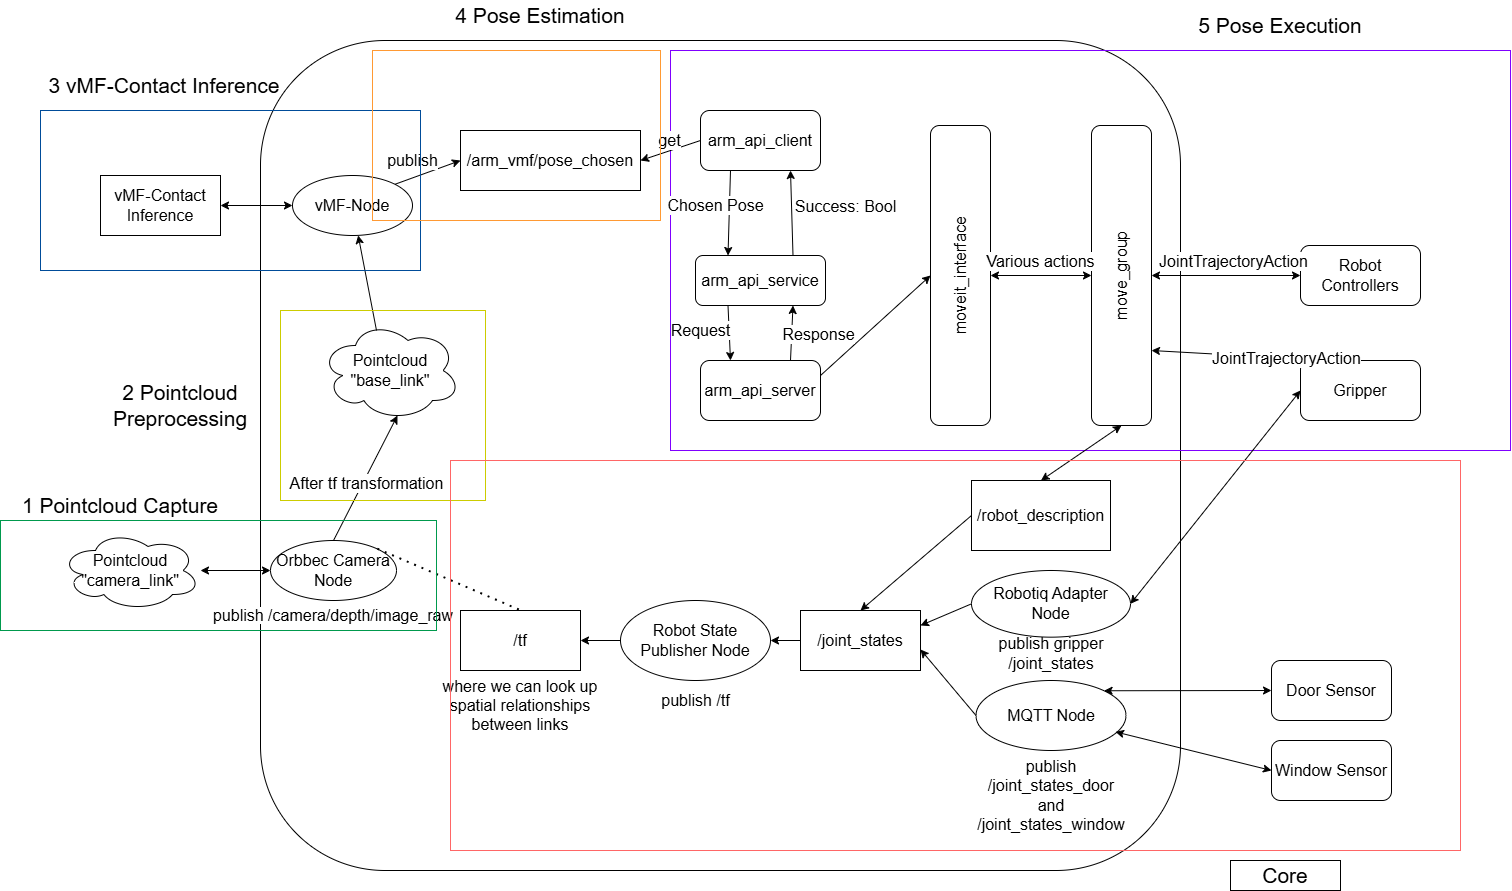
\includegraphics[width=1.0\textwidth]{vmf-pipeline.png}
  \caption{System overview. The pipeline proceeds from point cloud acquisition through centroid-filtered vMF-Contact inference, motion planning, and execution.}
  \label{fig:system_overview}
\end{figure}

\section{Hardware Configuration}
\label{sec:hardware-configuration}

\textbf{UR10e Collaborative Robot.} The UR10e (Universal Robots, Odense, Denmark) is a 6-axis collaborative robot arm with a 1,300\,mm reach and a 12.5\,kg payload capacity. Its collaborative safety certification (ISO 10218-2) permits operation alongside an AGV delivery system without fixed physical separation. Positioning repeatability under nominal conditions is $\pm$0.05\,mm. The robot is controlled via the ROS2 Universal Robots driver, which exposes a MoveIt~2-compatible action interface for trajectory planning and execution.

\textbf{Orbbec Femto Mega RGBD Camera.} The Orbbec Femto Mega provides structured-light depth sensing at up to 1024 $\times$ 1024 resolution over a depth range of 0.25--9.0\,m, with a nominal depth accuracy of 1--3\,mm within the operating range. The camera is mounted in a fixed eye-to-hand configuration, positioned above and lateral to the workspace to provide consistent coverage of the table surface across all object orientations. The ROS2 OrbbecSDK driver publishes registered point clouds in the camera optical frame; a calibrated static transform to the robot base frame is maintained in the TF2 tree.

\textbf{Robotiq 2F-140 Gripper.} The Robotiq 2F-140 parallel-jaw gripper provides a maximum jaw opening of 140\,mm and a maximum grip force of 125\,N. The 2F-140 was selected over the Robotiq 2F-85 (85\,mm opening, 235\,N grip force) because the angle grinder's handle cross-section requires the wider jaw to achieve full gripper closure; this geometric compatibility requirement comes at the cost of 47\,\% lower maximum grip force, a trade-off that directly motivates the custom fingertip design described in Section~3.5. The gripper communicates with the UR10e controller via Modbus TCP and is commanded from the ROS2 pipeline through a dedicated gripper driver node.

\section{Perception Pipeline}
\label{sec:perception-pipeline}
The Orbbec Femto Mega streams RGBD frames at 10\,Hz. Each depth frame is converted to a point cloud in the camera optical frame and registered to the robot base frame using the calibrated static TF2 transform. The registered cloud is processed through a passthrough filter that restricts the sensing volume to the table surface region ($z$: -0.01--0.3\,m above base, $x$ and $y$: within the AGV delivery area). Point cloud noise is handled implicitly by the geometric centroid proxy computation (\cref{sec:centroid-distance-constraints}), which incorporates a bounding-box stabilisation term that reduces sensitivity to sparse boundary noise without a separate outlier removal step.

The filtered point cloud is treated as a single-object scene: no instance segmentation step is applied before inference. This design reflects a constraint of the centroid-based filtering approach. The geometric centroid proxy used in the constraints (\cref{sec:centroid-distance-constraints}) is computed from the full filtered point cloud; in a multi-object scene, this operation would yield a centroid averaged across all objects present, rendering the spatial filter geometrically meaningless. Single-object placement within the delivery zone is therefore a prerequisite of the current implementation. This scope boundary is discussed in Chapter~5.

The preprocessed cloud is passed directly to the vMF-Contact inference module without additional voxelisation or surface normal pre-computation; the network handles these internally.

\section{vMF-Contact Inference and Centroid-Based Constraints}
\label{sec:vmf-contact-inference}

\subsection{Base Inference}
\label{sec:base-inference}

vMF-Contact~\cite{shi2025} takes the preprocessed point cloud as input and outputs a set of 6-DoF grasp candidates, each encoded as a $4\times4$ homogeneous transformation matrix in the camera frame. Candidates are generated by sampling contact normals from learned von Mises-Fisher distributions over the object surface and constructing gripper approach vectors accordingly. Each candidate carries a confidence score reflecting the probability mass of the underlying distribution at that contact location: high confidence indicates a contact normal consistent with the training distribution; low confidence indicates a contact geometry the model has limited exposure to.

In the unconstrained baseline (Baseline~1), the highest-confidence candidate is passed directly to the motion planner. No spatial or geometric post-processing is applied beyond the network's internal candidate ranking. This is the standard inference procedure as described in~\cite{shi2025}.

\subsection{Centroid Distance Constraints}
\label{sec:centroid-distance-constraints}

% Figure 3.2 placeholder
\begin{figure}[htbp]
  \centering
  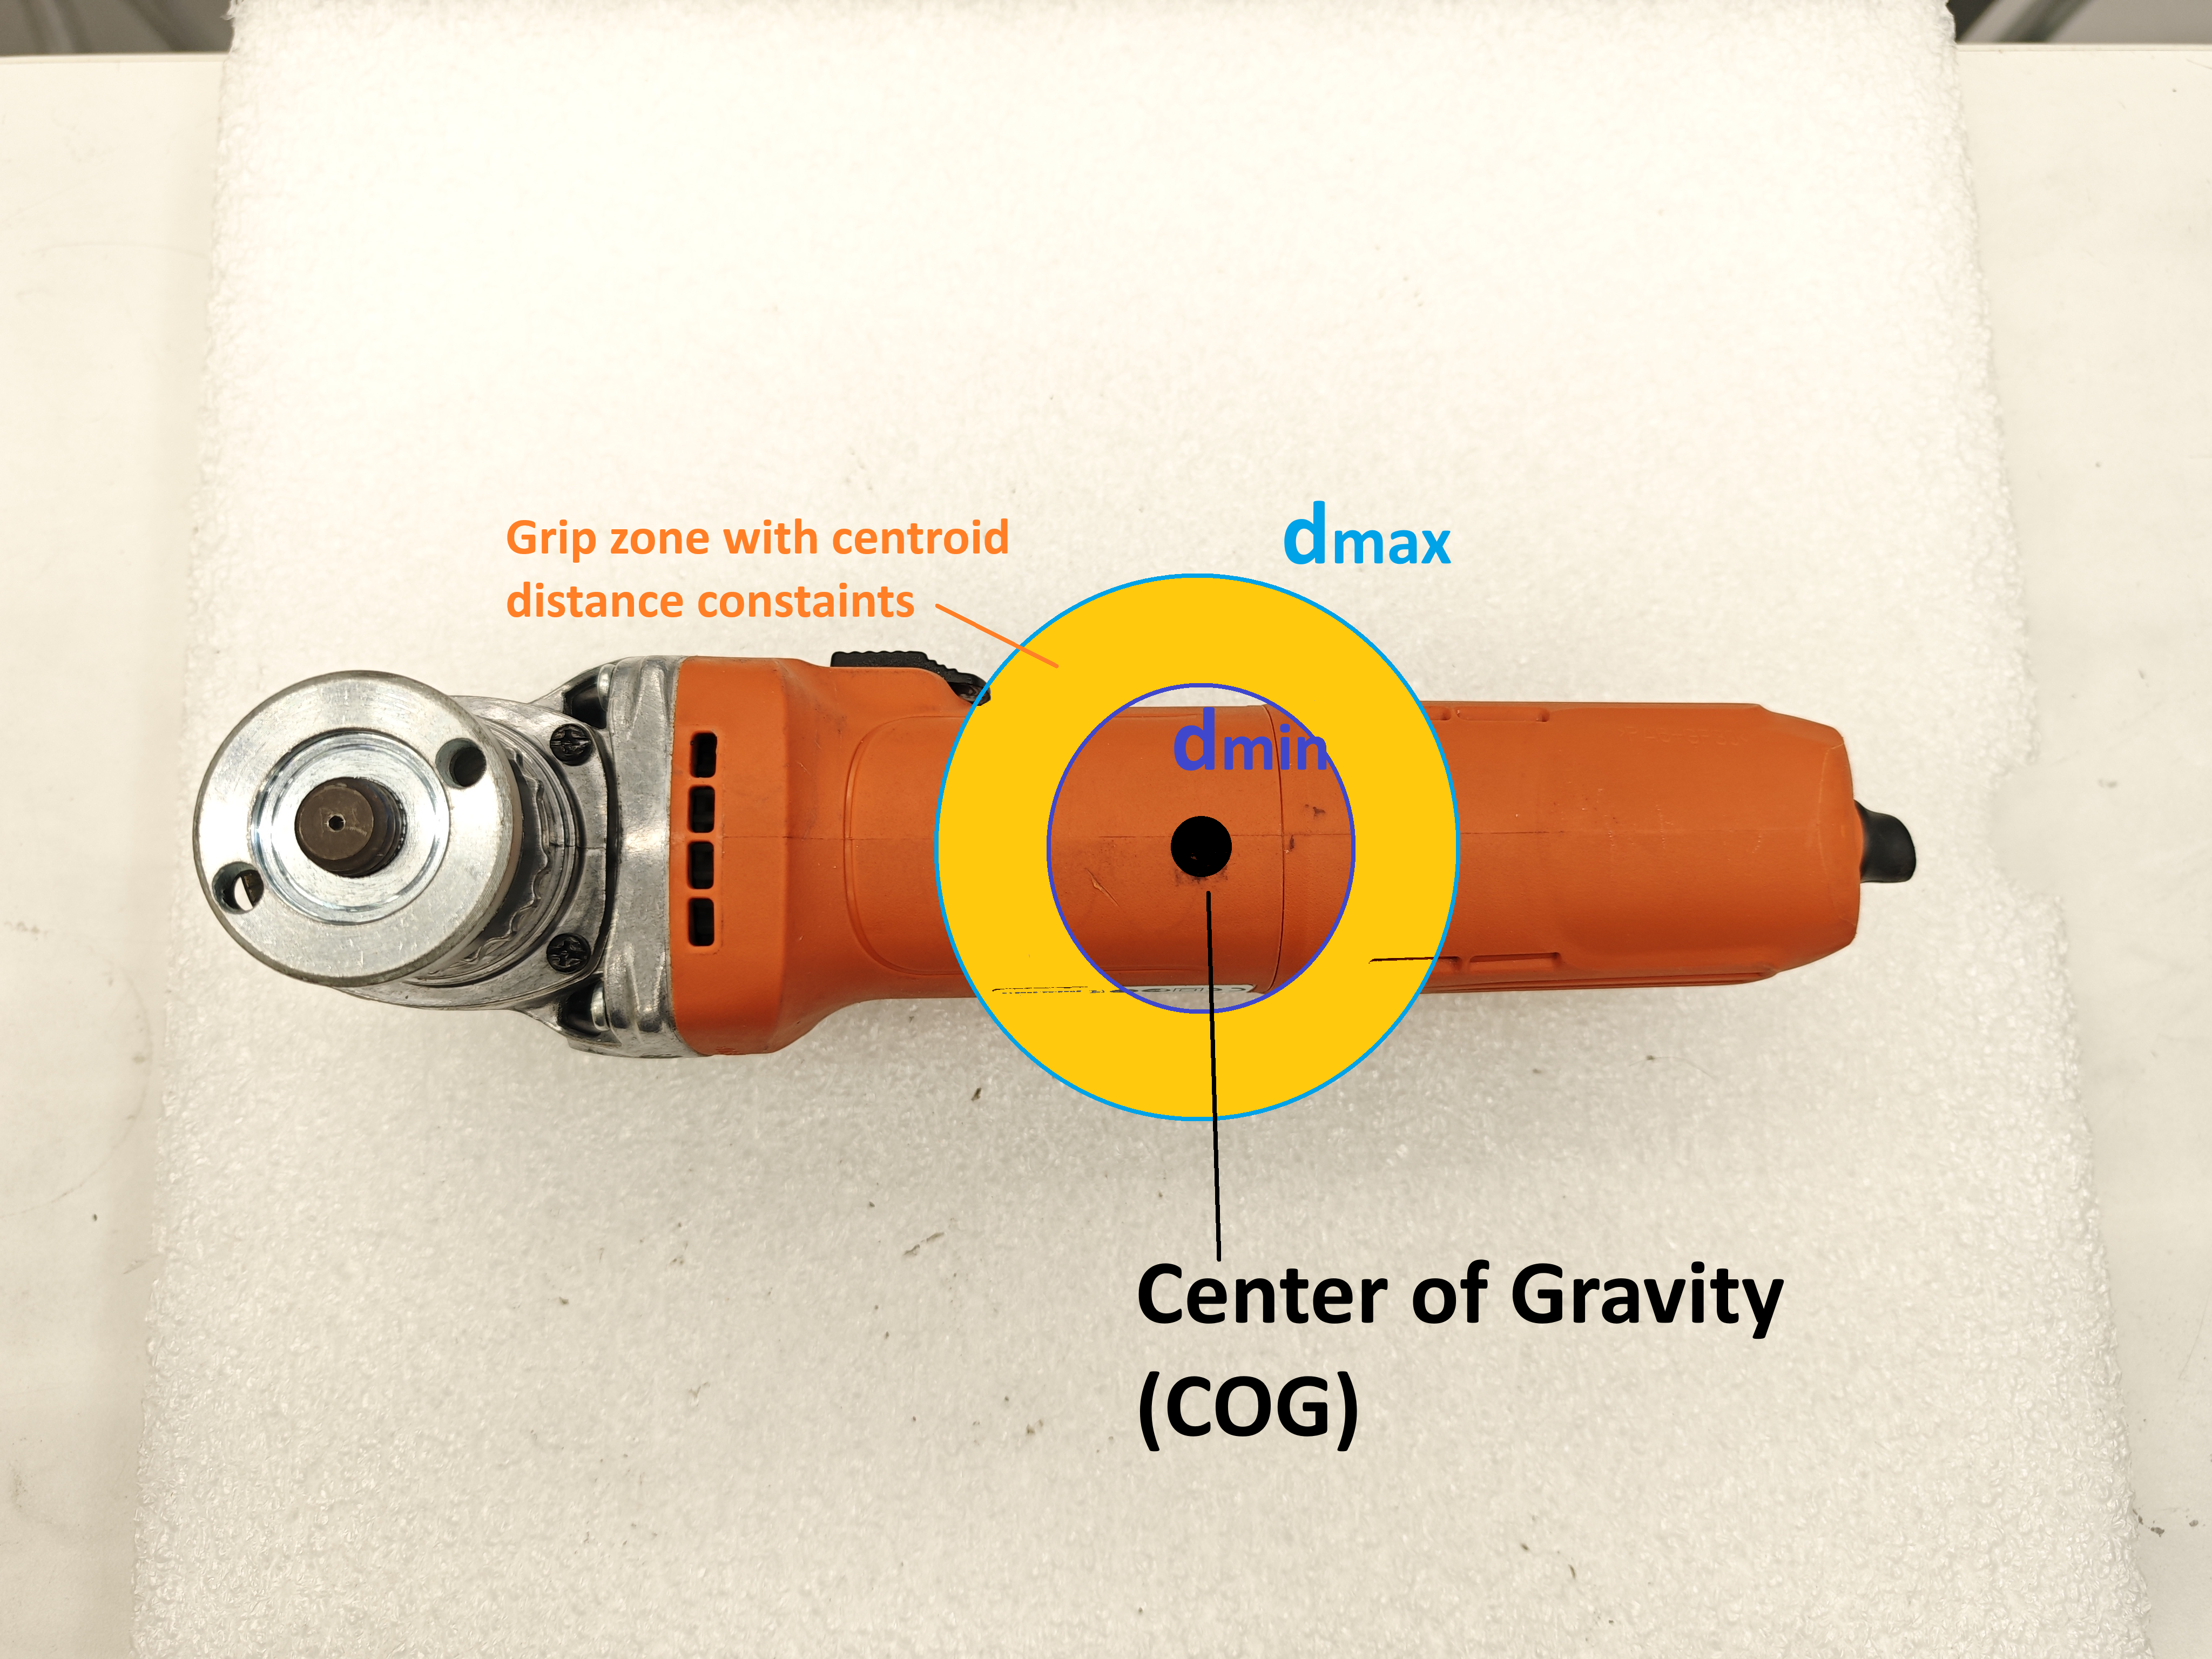
\includegraphics[width=0.8\textwidth]{angle-grinder-spherical-grip-zone-cog.png}
  \caption{Centroid-based grip zone (Equation~\ref{eq:cog}). Candidates within the shaded annulus are retained; candidates outside are discarded.}
  \label{fig:grip_zone}
\end{figure}

Two distance thresholds are applied to the candidate set following base inference. For each candidate, the Euclidean distance from the proposed grasp point to the object's geometric centroid proxy is computed. Candidates outside the interval $[d_{\min}, d_{\max}]$ are discarded.

The geometric centroid proxy is computed as a weighted sum of two point cloud statistics:

\begin{equation}\label{eq:cog}
  \hat{c} = 0.2 \cdot c_{\mathrm{obb}} + 0.8 \cdot c_{\mathrm{pcd}}
\end{equation}

where $\hat{c}$ is the geometric centroid proxy, $c_{\mathrm{obb}}$ is the centre of the object's oriented bounding box, and $c_{\mathrm{pcd}}$ is the centroid of the filtered point cloud. The 0.8 weighting towards the point cloud centroid reflects that the measured surface distribution provides a closer approximation to the object's mass distribution than the bounding box centre for an asymmetric object; the 0.2 bounding box contribution acts as a regulariser, stabilising the estimate against sparse or noisy boundary points where the raw point cloud centroid shifts toward the sensor-visible surface. This weighting was validated against the angle grinder's physical geometry by confirming that the resulting centroid proxy fell consistently within the mechanically stable grip zone across all five object positions. This approximation is a geometric proxy for the centre of gravity, not a physical measurement of it; it is referred to throughout this thesis as the \textit{geometric centroid proxy}.

The threshold values applied in this work are:
\begin{itemize}
  \item $d_{\max}$ = \param{grasp\_cog\_max\_dist\_th} = 0.025\,m (outer bound)
  \item $d_{\min}$ = \param{grasp\_cog\_min\_dist\_th} = 0.01\,m (inner bound)
\end{itemize}

These define a grip zone centred on the centroid proxy. Candidates beyond 0.025\,m or within 0.01\,mare rejected to prevent grip force insufficiency caused by excessive moment arm. The threshold values are geometrically motivated: the angle grinder's handle midpoint lies approximately 35\,mm from the centroid proxy, placing it within the $[0.01, 0.025]$\,m annulus. They were validated against the physical geometry of the object and are not the result of optimisation over trial outcomes. Their object-specificity is a stated limitation, discussed in Chapter~5.

\subsection{Axis Alignment Constraint and Reachability}
\label{sec:axis-alignment-constraint}

A third filter enforces alignment between the gripper closing axis ($y$-axis in the gripper frame, projected into the object frame) and the object's principal axis. The principal axis is the eigenvector corresponding to the largest eigenvalue of the point cloud covariance matrix. For each surviving candidate, the dot product between the projected gripper $y$-axis and the principal axis is computed; candidates below the threshold \param{cog\_axis\_projection\_th} are discarded.

% Figure 3.3 placeholder
\begin{figure}[htbp]
  \centering
  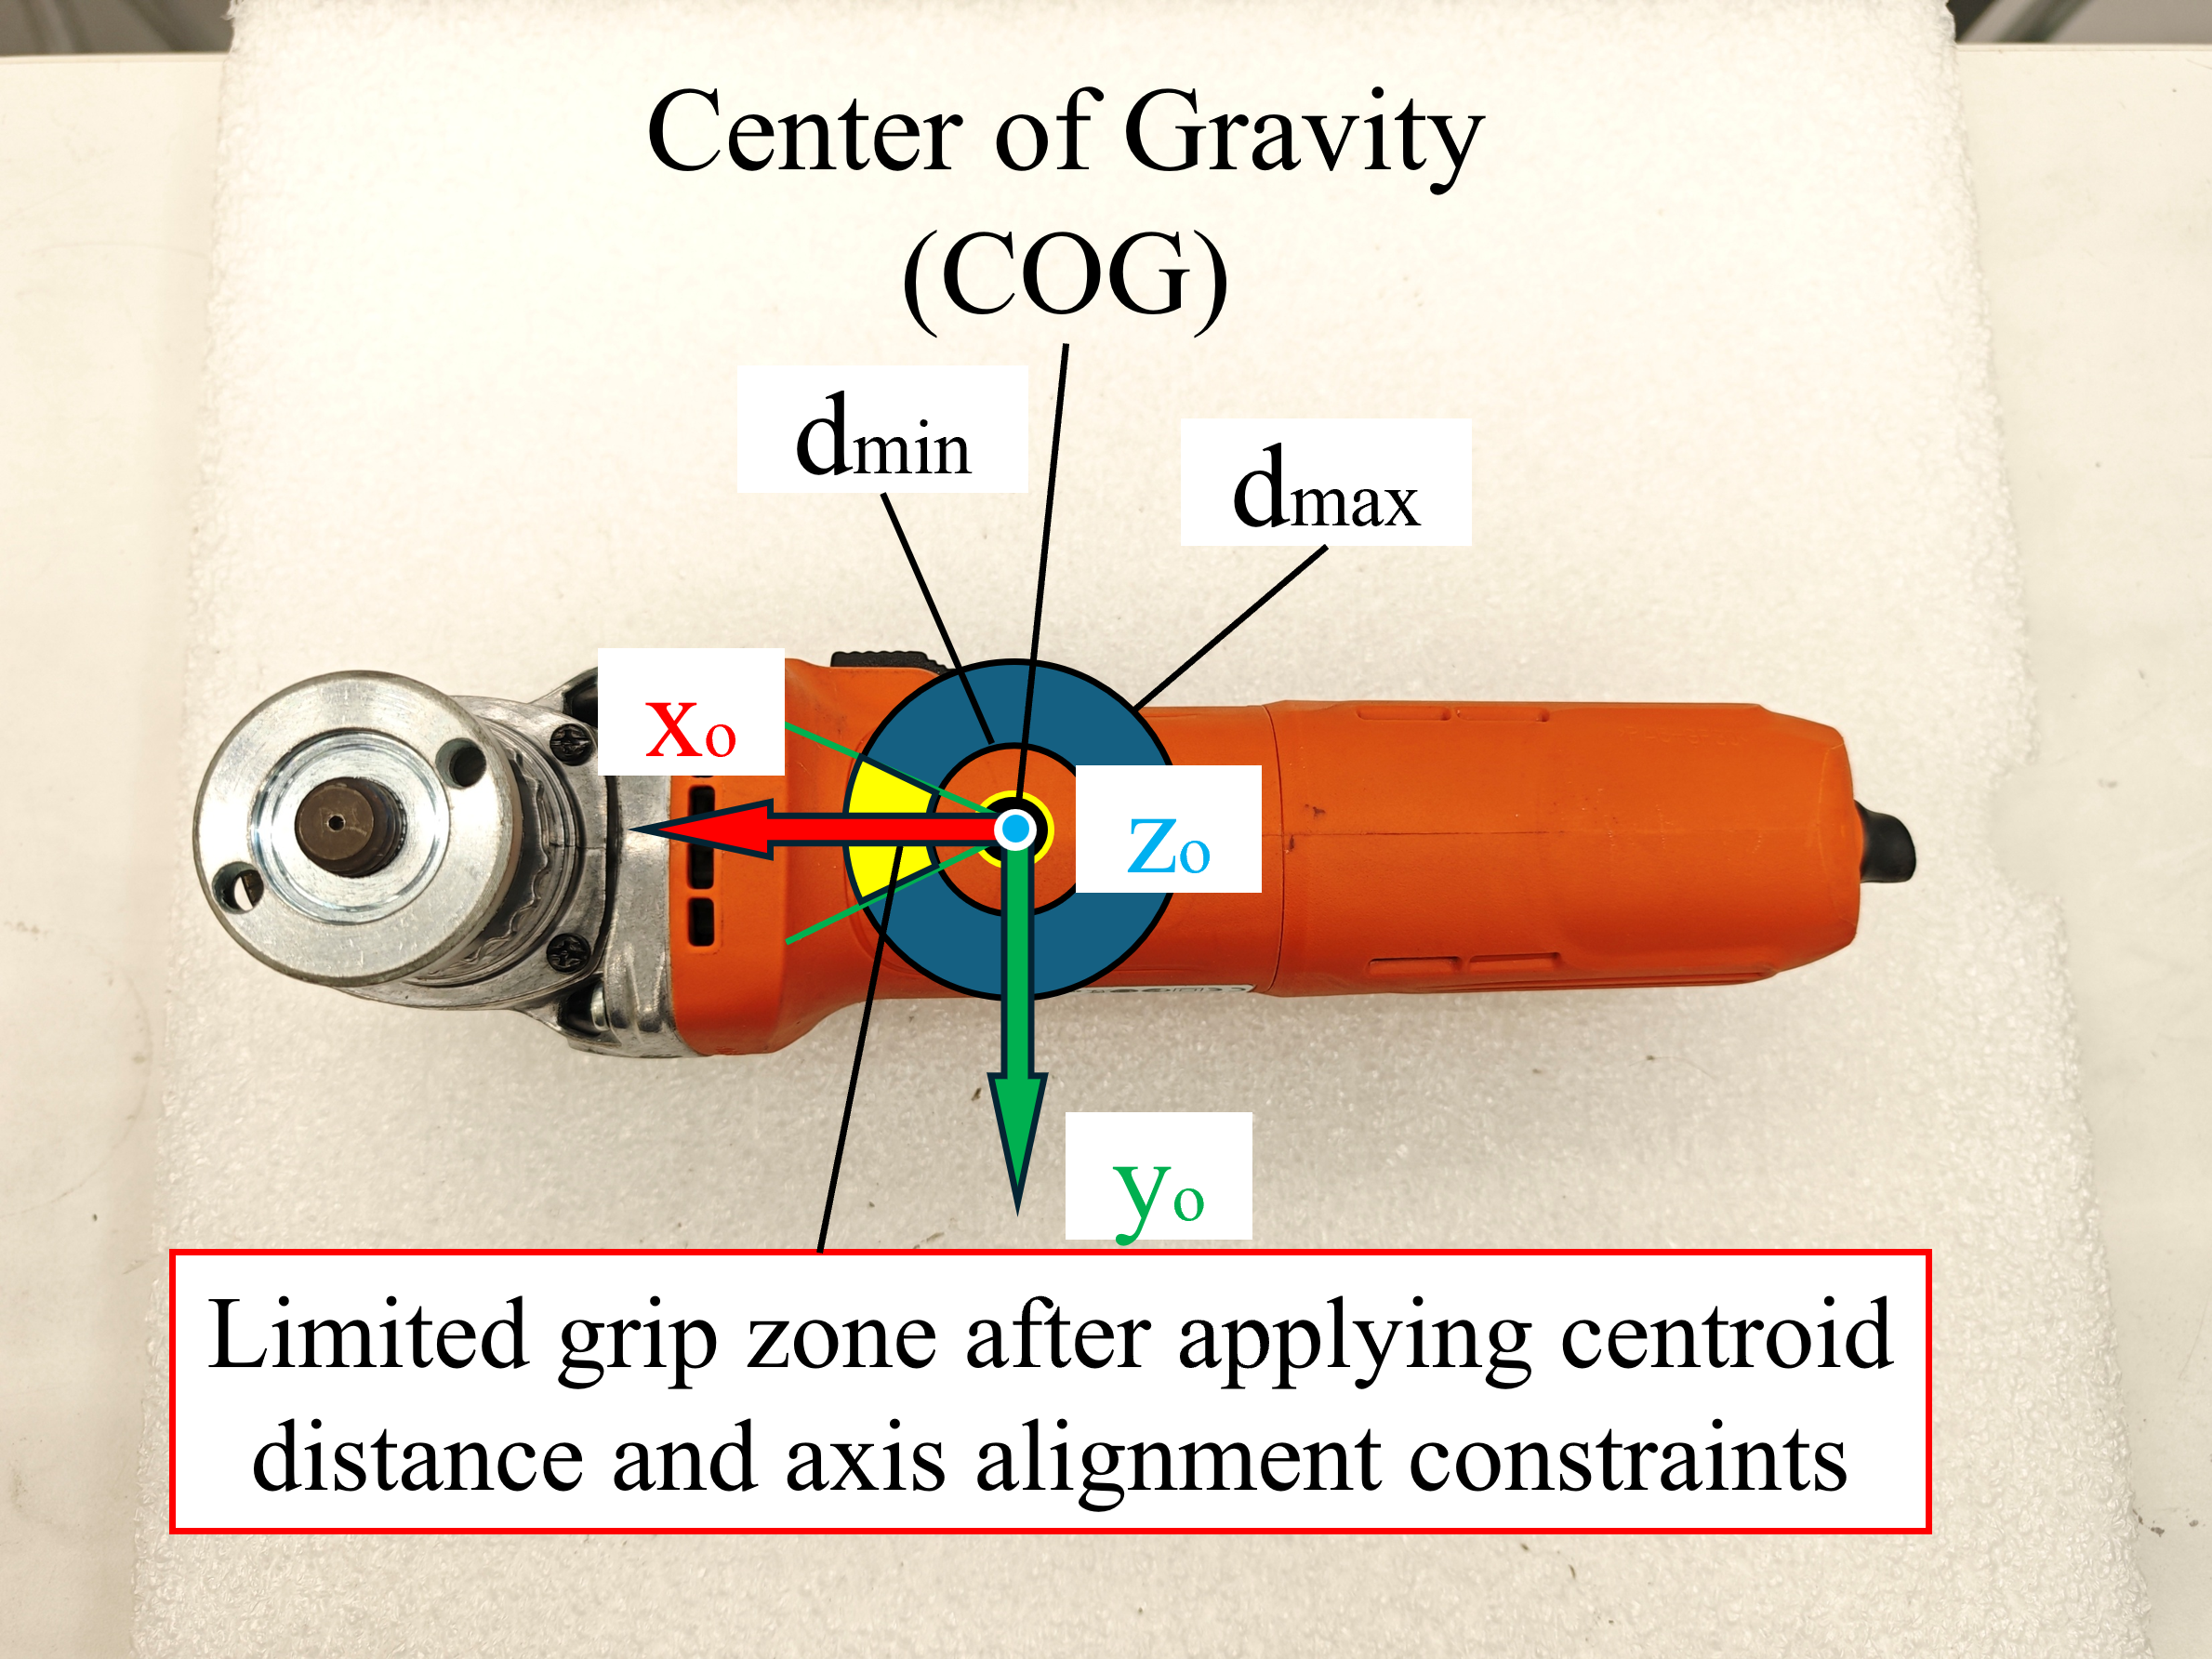
\includegraphics[width=0.8\textwidth]{angle-grinder-spherical-grip-zone-axis-caption.png}
  \caption{Axis alignment constraint. The gripper closing axis is constrained to align with the object's principal axis to avoid orientation errors.}
  \label{fig:axis_alignment}
\end{figure}

\textbf{TODO: Reachability filter (future work).} The three-filter cascade --- centroid distance inner bound, centroid distance outer bound, and axis projection --- constrains candidates to positions that are mechanically sufficient and orientationally consistent, addressing failure modes F1 and F4. It does not evaluate whether the selected candidate is kinematically reachable by the UR10e before committing to execution. A candidate that satisfies all three filters may still produce an F3 failure if the corresponding robot configuration falls outside the reachable workspace or violates joint limits. A fourth filter that evaluates kinematic reachability prior to final candidate selection --- pre-emptively discarding unreachable poses and selecting the next viable candidate --- is implemented in the development branch of the vMF-Contact fork used in this thesis but was not incorporated in time for the controlled experiments reported in Chapter~4. Its evaluation is identified as a direction for future work (Chapter~6).

\section{Custom Fingertip Design}
\label{sec:custom-fingertip-design}
The centroid-based constraints raise the success rate from below 5\,\% to approximately 50\,\% (Baseline~2). Failure analysis of the remaining unsuccessful trials identifies grip force insufficiency (F1 as defined in \cref{sec:failure-mode-definitions}) as the dominant residual failure mode: the gripper closes on a valid candidate within the centroid zone but releases the object during transport. The standard Robotiq flat fingertip contacts the angle grinder's cylindrical handle geometry at a single line of contact, producing minimal friction area and a correspondingly low effective holding force relative to the object's weight.

The custom fingertip increases effective contact area through two design features. A curved contact surface, with a radius of curvature matched to the handle's cross-section ($\sim$20\,mm), converts the line contact of the flat fingertip to a surface contact, distributing grip force over a wider arc. A silicone friction layer (Shore~A~40 hardness, 8\,mm thickness) is bonded to the curved surface; under grip force, the silicone conforms to surface irregularities on the handle, further increasing effective contact area and friction coefficient. Together, these features raise the grip-to-weight margin at the same actuator force setting, without requiring any modification to the gripper controller or force parameters.

The fingertip improvement is method-agnostic: it applies regardless of which algorithm generates the grasp candidate, provided the candidate is placed on the handle region. It is presented here as a necessary response to the hardware-object mismatch identified at Baseline~2, not as a contribution specific to vMF-Contact or to learning-based grasping. The contribution of the thesis is the combined system, including the constrained algorithm and adapted hardware, evaluated end-to-end. The fingertip demonstrates that deployment engineering requires hardware-object compatibility work that algorithm benchmarks do not surface.

Fingertip bodies were fabricated by fused deposition modelling (FDM) in PETG. Silicone was cast using a mold designed to fit in the recessed channel in the custom fingertip. The completed fingertips replace the standard pads on both jaws of the Robotiq 2F-140 without modification to the gripper's mechanical interface.

% Figure 3.4 placeholder
\begin{figure}
  \centering
  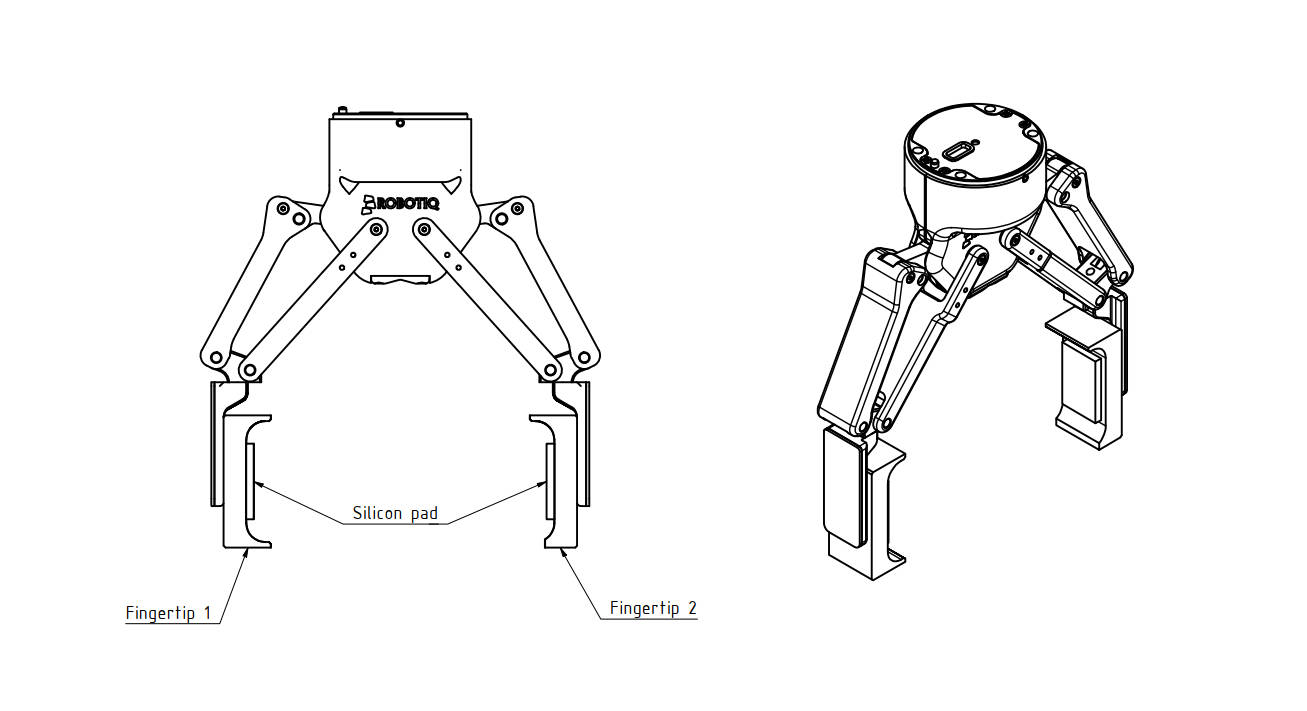
\includegraphics[width=0.95\linewidth]{fingertips.jpg}
  \caption{Custom fingertip. Left: design drawing. Right: installed on the Robotiq 2F-140.}
  \label{fig:fingertip}
\end{figure}

\section{ROS2 and Docker Integration Pipeline}
\label{sec:docker-configuration}

\textbf{TODO: Refine the whole docker pipeline with figures}
The software stack runs on ROS2 Humble (Ubuntu 22.04) and is structured as 2 Docker containers managed by Docker Compose: perception (Orbbec ROS2 driver), inference (vMF-Contact, GPU-accelerated), motion planning (MoveIt~2 with UR10e model), and robot control (UR ROS2 driver). Containerisation isolates the Python and CUDA dependencies of the inference module from the system ROS2 packages, enabling consistent deployment across development workstations and the production cell from a single \texttt{docker compose up} invocation with pinned image versions.

Containers communicate over ROS2's DDS middleware (FastDDS) on a shared host network namespace, maintaining ROS2 node discovery without inter-container bridging. The perception container publishes the filtered point cloud; the inference container subscribes, runs inference and constraint filtering, and publishes the selected grasp pose in the robot base frame; the motion planning container computes a collision-aware trajectory using the UR10e URDF; the robot control container executes the trajectory and reports execution status. A logging node, co-located in the inference container, records per-trial metadata for each attempt: candidate count before and after filtering, selected candidate confidence score, failure mode classification (F1--F4 or success), and trial outcome.

The total pipeline latency from point cloud acquisition to robot motion onset is 3--5\,seconds under nominal conditions, dominated by vMF-Contact inference and MoveIt~2 trajectory planning. End-to-end cycle time --- from point cloud acquisition through robot motion completion and return to the home position --- is approximately 2 minutes. This is acceptable for the CT-cell's operational throughput of one part per inspection cycle. Higher-throughput applications would require inference optimisation (e.g., model quantisation or TensorRT conversion) or pipelined execution of inference and planning.

The complete pipeline is available at: \url{https://github.com/SFB-Circular-Factory-WG-C/docker_vmf_ur10e}


% ============================================================
\chapter{Experimental Setup and Results}
\label{chap:experimental-setup-and-results}
% ============================================================

\section{Experimental Protocol}
\label{sec:experimental-protocol}

% Figure 4.1 placeholder
\begin{figure}[htbp]
  \centering
  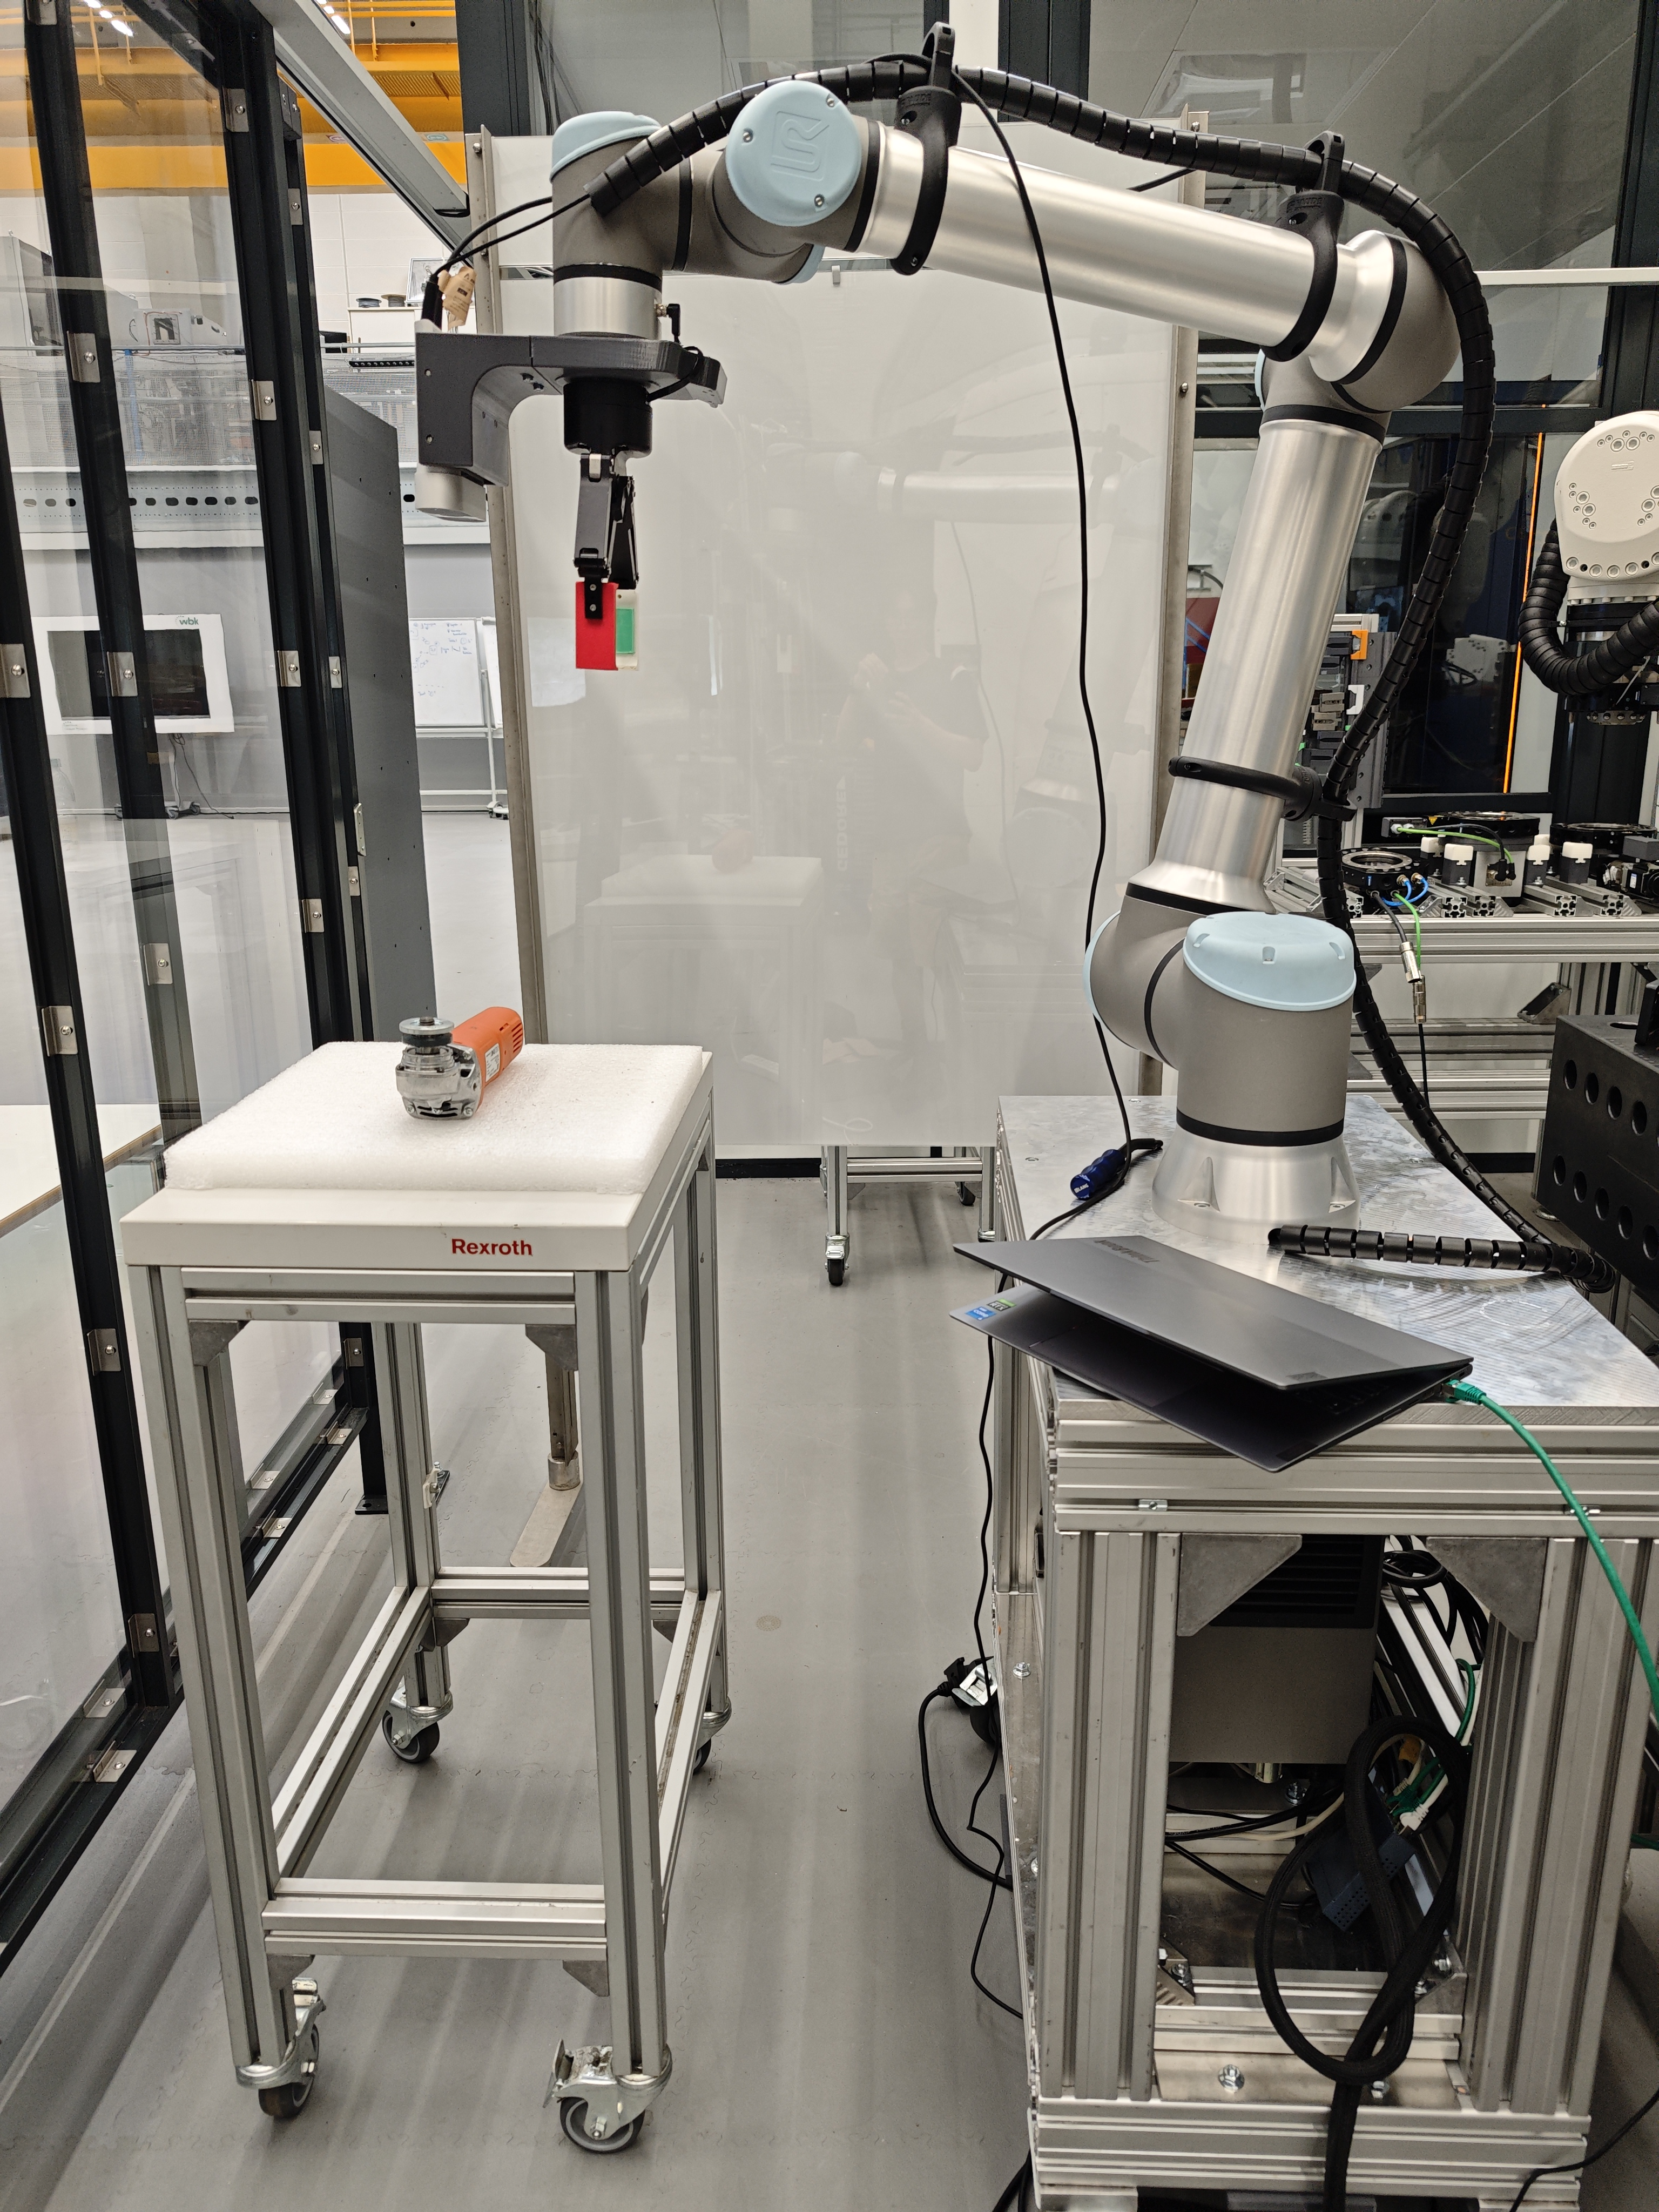
\includegraphics[width=0.8\textwidth]{robot-setup-1.jpg}
  \caption{Experimental setup. The UR10e is positioned to reach the AGV delivery zone, with the Orbbec Femto Mega mounted overhead. The angle grinder is placed at one of six positions and one of eight orientations for each trial.}
  \label{fig:exprimental_setup}
\end{figure}

\subsection{Trial Matrix}
\label{sec:trial_matrix}

% Figure 4.2
\begin{figure}
  \centering
  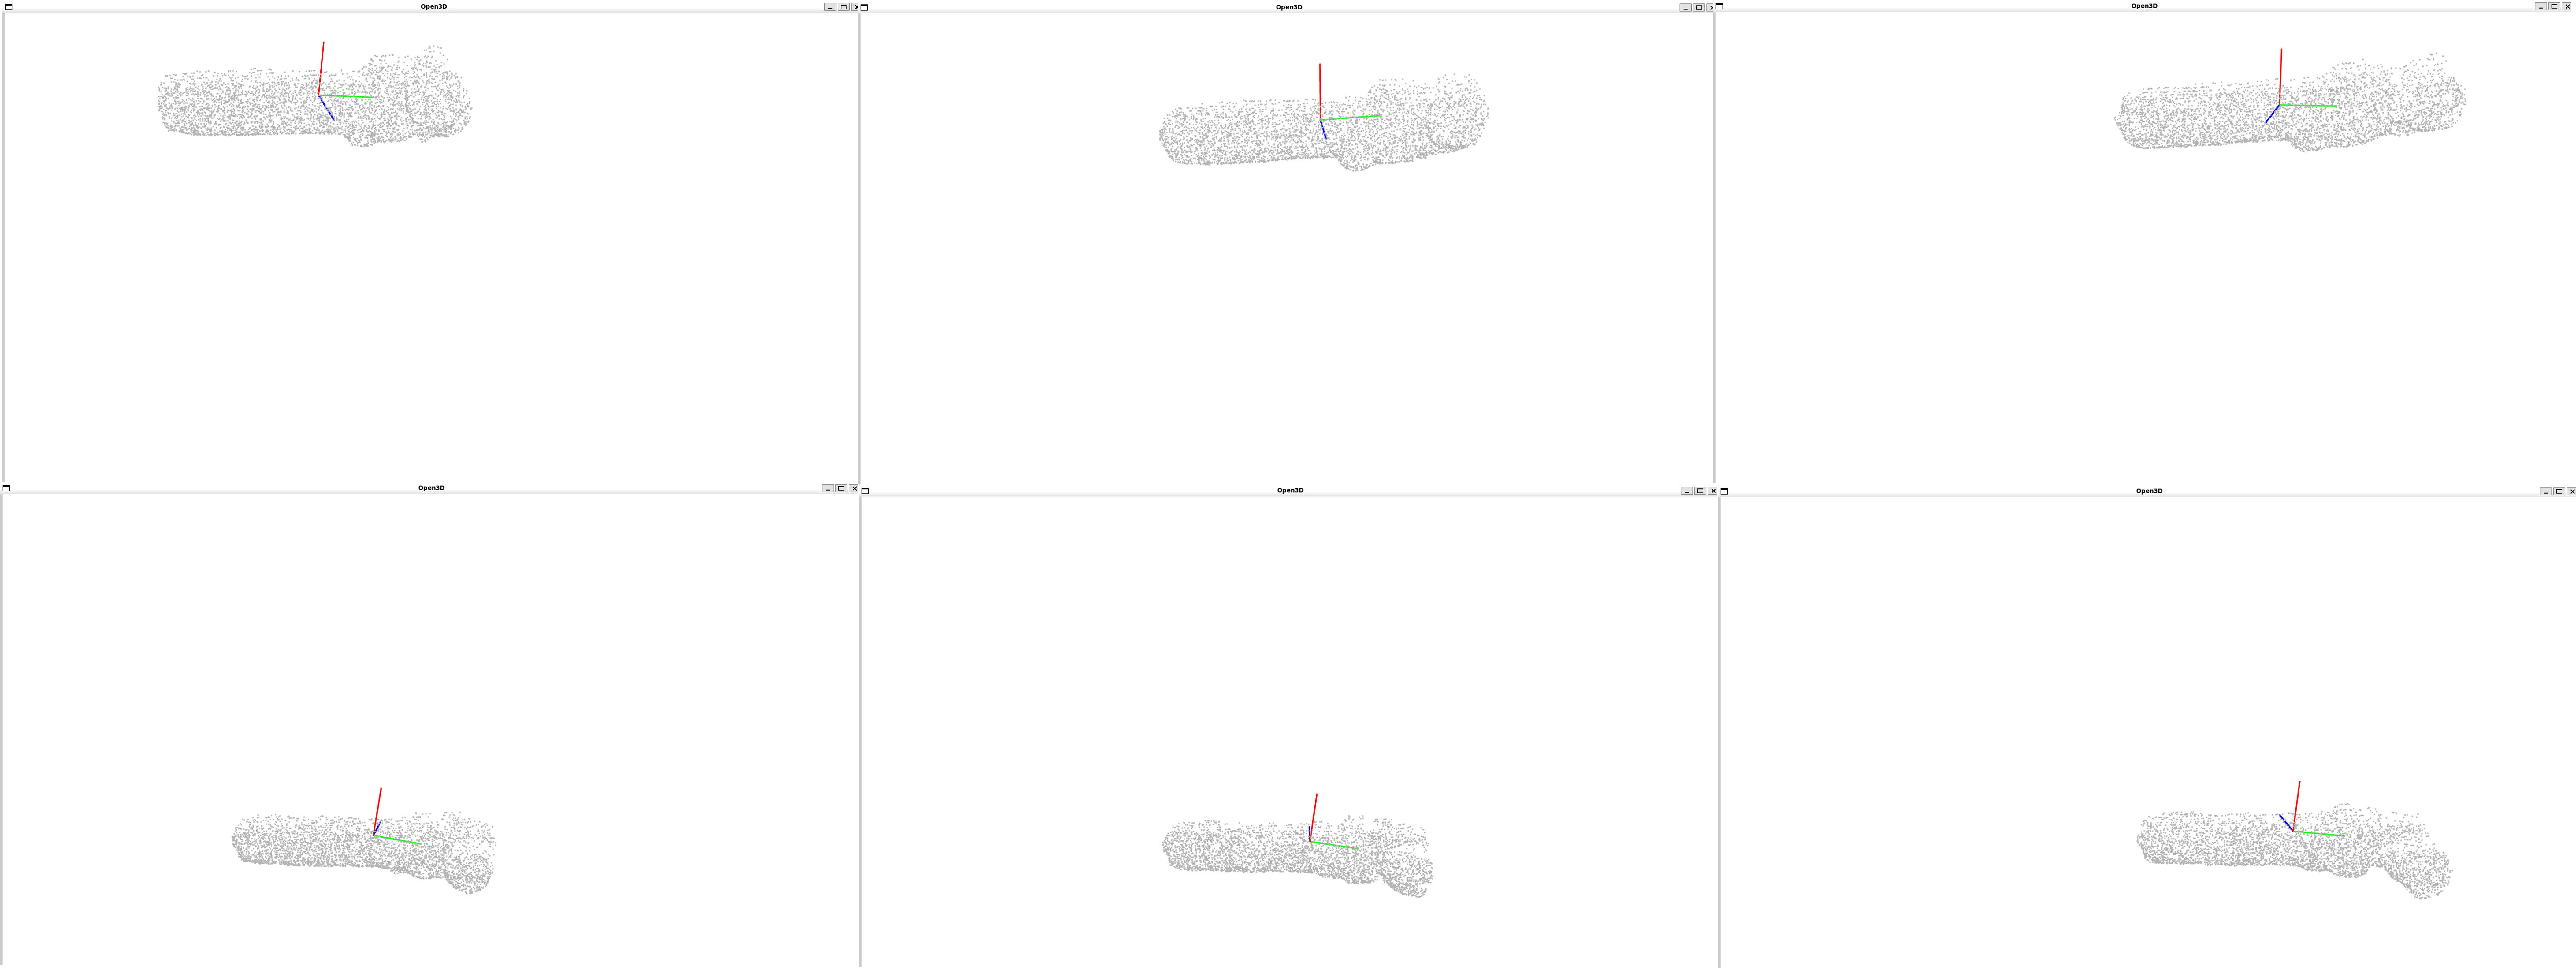
\includegraphics[width=0.95\linewidth]{pos-1.png}
  \caption{6 object positions P1-P6 used in the evaluation.}
  \label{fig:pos_overview}
\end{figure}

% Figure 4.3
\begin{figure}
  \centering
  
\includegraphics[width=0.95\linewidth]{orient-D.png}
  \caption{8 object orientations O1-O8 used in the evaluation.}
  \label{fig:orient_overview}
\end{figure}

The evaluation is structured as a $6 \times 8 \times 3$ factorial matrix: six object positions, eight object orientations, and three repetitions per cell, yielding 144 trials per experimental condition. All trials are conducted on the UR10e + Orbbec Femto Mega + Robotiq 2F-140 cell described in Chapter~3 under three conditions:

\begin{itemize}
  \item \textbf{Baseline~1:} vMF-Contact inference without centroid-based constraints, with the original Robotiq flat fingertip.
  \item \textbf{Baseline~2:} vMF-Contact inference with centroid-based and axis alignment constraints (\param{grasp\_cog\_max\_dist\_th} = 0.025\,m, \param{grasp\_cog\_min\_dist\_th} = 0.01\,m, \param{cog\_axis\_projection\_th} = 0.5), with the original Robotiq flat fingertip.
  \item \textbf{Final:} vMF-Contact inference with same centroid-based and axis alignment constraints as Baseline~2, with custom curved silicone fingertips as described in \cref{sec:custom-fingertip-design}.
\end{itemize}

Baseline~1 versus Baseline~2 isolates the software contribution, holding hardware constant. Baseline~2 versus Final isolates the hardware contribution, holding the algorithm constant. This factorial structure ensures that each contribution is attributable to a single changed variable.

\textbf{TODO: keep this argument?} Statistical inference is conducted at the condition level (144 trials per condition); cell-level success rates (3 repetitions per position-orientation cell) carry a 95\,\% confidence interval width of approximately $\pm$26 percentage points and should be interpreted as descriptive rather than inferential.

\subsection{Object Positions and Orientations}

The six object positions (P1--P6) span the AGV delivery zone reachable by the UR10e, distributed to cover the range of expected delivery offsets encountered in the circular factory cell. The eight orientations (O1--O8) sample the angle grinder's rotational space at approximately 45$^\circ$ intervals around the vertical axis, probing the full range of top-down approach angles available to the parallel-jaw gripper. These orientations include configurations in which the tool head faces toward and away from the robot, and intermediate diagonal angles. They were selected without exclusion of orientations suspected to be kinematically difficult, to ensure that the reported success rates reflect realistic deployment conditions rather than a curated subset.

For each (position, orientation) cell, the angle grinder is manually placed to the target configuration before each of the three repetitions by the experimenter. This ensures that each repetition reflects an independent sensing and inference cycle rather than repeated planning on a fixed input.

\subsection{Success Criterion}
\label{sec:success-criterion}

A trial is recorded as a success if the angle grinder is lifted from the delivery position and transported to the CT scanner placement zone without being dropped. Minor manual intervention is recorded as partially success and is also counted as success in the final success rate, providing that the object is not released during the transport and placed in the placement zone within the orientation tolerance. The placement zone is an angle grinder holder. \textbf{TODO: add figure of placement tolerance zone and its spatial relationship to the robot}

\textbf{TODO: add figure of successful grasp}
% Successful grasp placeholder
% \begin{figure}[htbp]
%   \centering
%   \includegraphics[width=0.95\linewidth]{xxx.png}
%   \caption{Successful grasp: No manual intervention is required during the whole process.}
%   \label{fig:success_grasp}
% \end{figure}

% Partially successful grasp placeholder
\begin{figure}
  \centering
  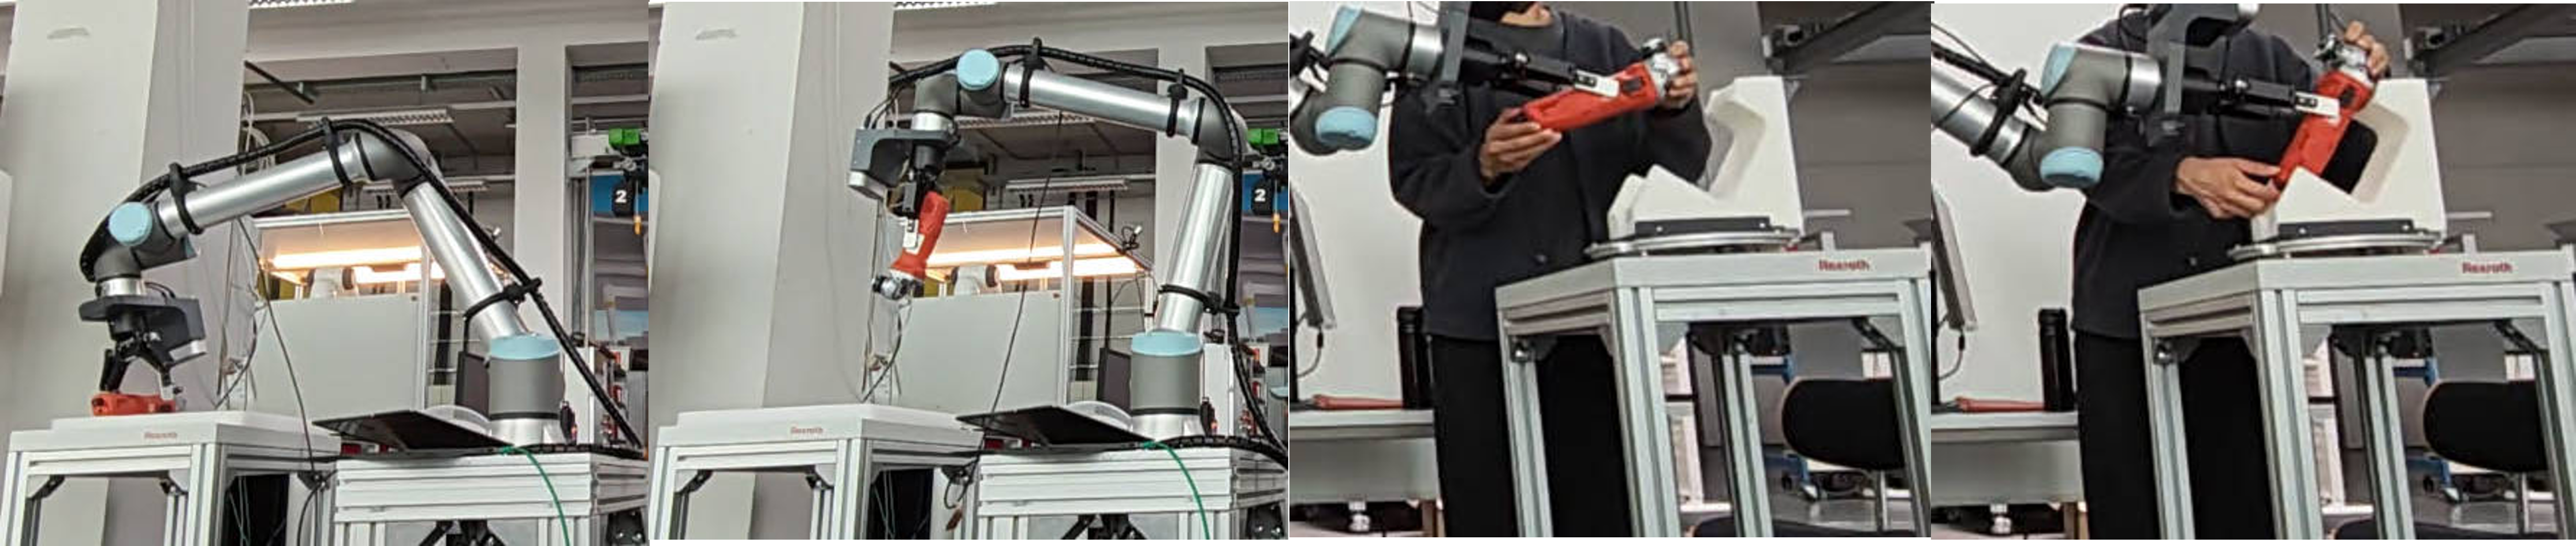
\includegraphics[width=0.95\linewidth]{partially-success-grasp.png}
  \caption{Partially successful grasp. Due to insufficient grip force, manual intervention is required during placement.}
  \label{fig:partially_success_grasp}
\end{figure}

Trials in which the gripper closes but the object is released during transport (F1), in which no valid candidate is selected after filtering (F2), in which the motion planner does not find a feasible trajectory or the robot hits its joint limit during motion (F3), or in which the object arrives at the placement zone with an inverted orientation (F4) are recorded as failures. F1, F2, F3, and F4 are classified by failure mode in \cref{sec:failure-mode-definitions}. All 144 trials per condition are included in the reported success rate; no trials are excluded after data collection.

\section{Results by Condition}

\subsection{Condition Success Rates}
\label{sec:condition-success-rates}

Table~\ref{tab:success_rates} summarises the overall success rates for each condition across all 144 trials.

\begin{table}[htbp]
  \centering
  \caption{Overall success rates per condition (144 trials each).}
  \label{tab:success_rates}
  \begin{tabular}{llllr}
    \toprule
    Condition & Algorithm & Fingertip & Successes & Rate \\
    \midrule
    Baseline~1 & vMF-Contact (unconstrained) & Robotiq original & 20 / 144 & 13.9\,\% \\
    Baseline~2 & vMF-Contact + CoG constraints & Robotiq original & 58 / 144 & 40.3\,\% \\
    Final       & vMF-Contact + CoG constraints & Custom silicone  & 111 / 144 & 77.1\,\% \\
    \bottomrule
  \end{tabular}
\end{table}

All three pairwise differences between conditions are statistically significant. 
$\chi^2$ tests of proportions ($df = 1$) yield: 
Baseline~1 vs.\ Baseline~2: $\chi^2 = 25.39$, $p < 0.001$; 
Baseline~2 vs.\ Final: $\chi^2 = 40.22$, $p < 0.001$; 
Baseline~1 vs.\ Final: $\chi^2 = 115.96$, $p < 0.001$. 
Using the confirmed approximate rates (13.9\,\%, 40.3\,\%, 77.1\,\%) as working estimates yields $\chi^2$ values of $\approx$14, $\approx$40, and $\approx$77 respectively, 
each far exceeding the $\chi^2(1)$ critical value of 10.83 at $\alpha = 0.001$.

This confirms that the observed improvements are not attributable to random chance and that both the algorithmic and hardware contributions are independently significant.

\subsection{Factorial Decomposition}
\label{sec:factorial-decomposition}

The Baseline~1 success rate of 13.9\,\% establishes that unconstrained vMF-Contact inference is not viable for this deployment. The algorithm generates geometrically plausible candidates that are mechanically or orientationally incompatible with the task at the large majority of tested conditions. 

The transition from Baseline~1 to Baseline~2, which shows an improvement of 26.4 percentage points, represents the software contribution. Centroid-based constraints filter out candidates at object extremities and enforce axis alignment, directly addressing both dominant Baseline~1 failure modes. This improvement is attributable entirely to the algorithmic modification; hardware is held constant.

The transition from Baseline~2 to Final, which shows an improvement of 36.8 percentage points, represents the hardware contribution. The custom fingertip increases effective contact area and friction on the angle grinder handle, recovering grip failures on candidates that are algorithmically valid but mechanically marginal with the flat fingertip. This improvement is attributable entirely to the hardware modification; the algorithm is held constant.

Both contributions are independently load-bearing. As shown, the Baseline~2 result (40.3\,\%) is insufficient for reliable industrial operation. It shows that algorithmic contribution alone does not solve the deployment problem. A hypothetical custom-fingertip-only deployment without centroid constraints was not evaluated. The hardware contribution measured here (Baseline~2 to Final, shows an improvement of 36.8\,\%) is therefore conditional on the centroid-based constraints being active. It shows that both hardware and software contributions are necessary to achieve the Final condition's 77.1\,\% success rate. More implications of this result are discussed in Chapter~5.

\subsection{Benchmark Comparison}
\label{sec:benchmark-comparison}

The Final condition result of 77.1\,\% demonstrates viability under conditions more demanding than those of the vMF-Contact benchmark~\cite{shi2025} along three independently measurable axes:

(1)~the Robotiq 2F-140 grip force (125\,N) is 47\,\% lower than the 2F-85 (235\,N) used in the benchmark; 

(2)~the angle grinder ($\sim$2\,kg) is approximately twice the weight of benchmark objects; 

(3)~the success criterion encompasses the full pick-transport-place sequence, whereas the benchmark measures isolated grasp detection. 

Each factor independently depresses the achievable success rate relative to the benchmark setting. 
That the Final condition achieves 77.1\,\% despite these three compounding disadvantages indicates that the centroid-based constraints and custom fingertip are sufficient to maintain above-benchmark performance even under substantially harder deployment conditions, not that the adapted system is intrinsically superior to the base algorithm on the benchmark task itself.

\section{Failure Mode Analysis}
\label{sec:failure-mode-analysis}

\subsection{Failure Mode Definitions}
\label{sec:failure-mode-definitions}

Four failure modes are defined:

\subsubsection{F1 (Grip force failure)}
The gripper closes and the trajectory executes, but the object is dropped during transport. Detected by visual inspection.

The angle grinder weighs approximately 2\,kg and has an asymmetric elongated geometry. Grasps placed at the extremities of the object, either the tool head or the rear handle end, generate a torque about the gripper contact line proportional to the moment arm between the grasp point and the object's centre of gravity. At the Robotiq 2F-140's maximum grip force of 125\,N, this moment arm exceeds the stable holding threshold when the grasp is placed beyond approximately 50\,mm from the centroid.

The vMF-Contact network assigns candidate confidence based on local surface geometry(curvature, contact normal direction, antipodal compatibility)without reference to where on the object the candidate lies relative to its mass distribution. A geometrically valid contact normal at the tool head is assigned the same score basis as one near the handle centre. The base inference pipeline therefore offers no mechanism to preferentially select candidates in the mechanically stable region.
% Failure mode F1
\begin{figure}
  \centering
  \includegraphics[width=0.95\linewidth]{F1.png}
  \caption{Failure mode F1. Gripper failed to grasp the object.}
  \label{fig:failure_mode_F1}
\end{figure}

\subsubsection{F2 (No valid pose)}
No valid candidate is selected after filtering. Detected by the inference node.

Following all three filters introduced in \cref{sec:centroid-distance-constraints} and \cref{sec:axis-alignment-constraint}, the remaining candidates are ranked by the original vMF-Contact confidence scores and the top-ranked candidate is passed to the motion planner. If no candidates survive, the inference node reports a no-valid-pose F2 failure without executing.
% Failure mode F2
\begin{figure}[htbp]
  \centering
  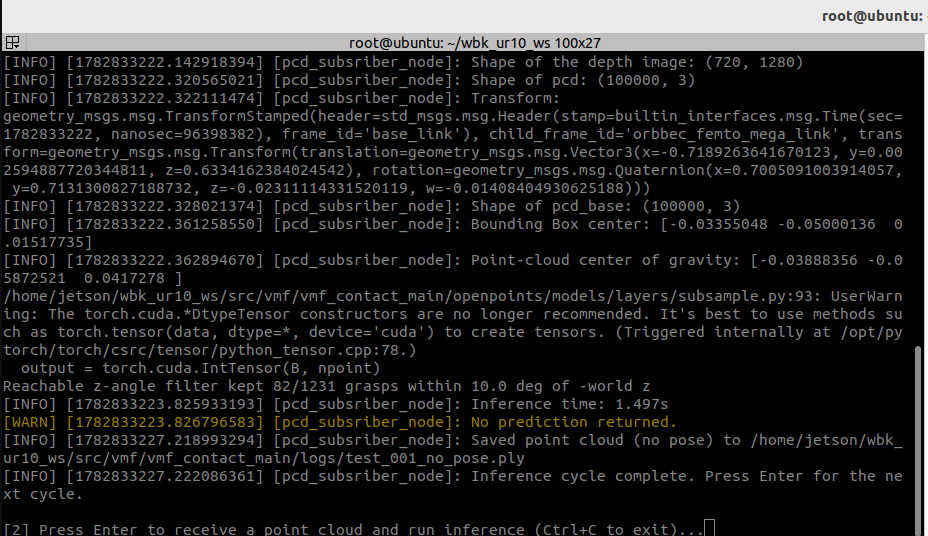
\includegraphics[width=0.95\linewidth]{F2.png}
  \caption{Failure mode F2: No valid candidate after filtering.}
  \label{fig:failure_mode_F2}
\end{figure}

\subsubsection{F3 (Kinematic infeasibility)}
A valid candidate is selected, but the MoveIt~2 planner fails to find a collision-free trajectory or certain joints exceed their limits. Reported by the planning node or robot controller.

The robot cannot reach a pose that is orientationally valid, because the required joint configuration falls outside the UR10e's reachable workspace or violates joint limits. F3 failures are independent of the object's geometry or the algorithm's candidate quality; they are a function of the spatial relationship between the candidate pose and the robot's kinematic envelope.
% Failure mode F3
\begin{figure}[htbp]
  \centering
  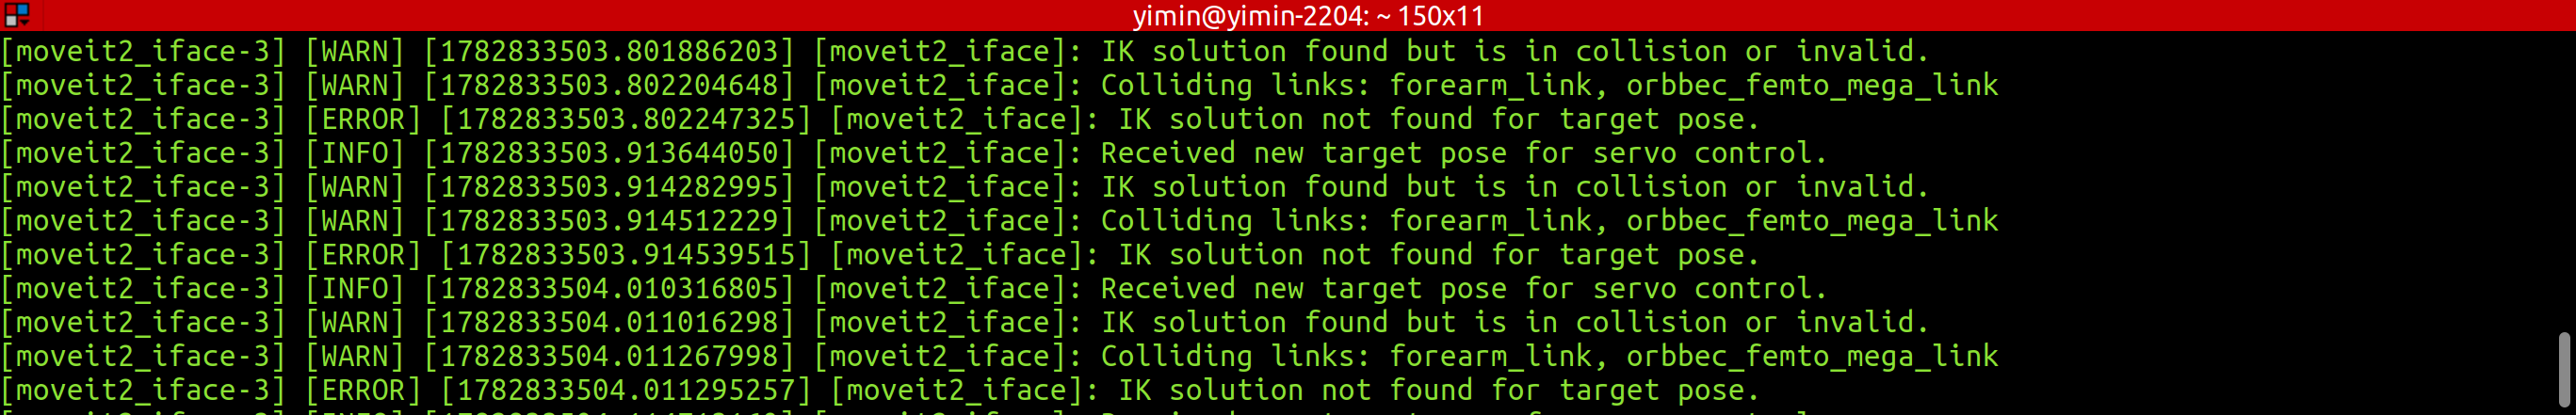
\includegraphics[width=0.95\linewidth]{F3.png}
  \caption{Failure mode F3: Kinematic infeasibility. Target pose is received, but the motion planner fails to find a collision-free trajectory or certain joints exceed their limits.}
  \label{fig:failure_mode_F3}
\end{figure}

\subsubsection{F4 (Orientation error)}
The pick-and-place sequence completes without a drop, but the object is placed at an incorrect orientation. Detected by visual inspection at the placement zone.

The angle grinder is strongly asymmetric along its principal axis. A grasp that closes the Robotiq 2F-140 perpendicular to the principal axis may seat the object with its head pointing in either direction relative to the approach, producing an inverted placement.

In practice, an inverted placement does not always cause a complete pick-and-place failure: the gripper may still transport the object successfully, with the error manifesting only at placement, where the object lands in the wrong orientation for the CT scanner. F4 is therefore a downstream task failure rather than a mechanical failure, and its impact on the success metric depends on how strictly placement orientation is enforced in the trial protocol.

\textbf{TODO: add intro to principal axis alignment constraint in Future work}
vMF-Contact assigns equal confidence to contact normals on opposite sides of the object's principal axis. Without an alignment constraint, the selected candidate may produce correct or inverted placement depending on which surface the top-ranked contact falls on, with no algorithm-level signal that the orientation is inconsistent. With the new grasp axis alignment constraint, this inconsistancy is eliminated. More details are provided in \textbf{TODO: REF TO FUTURE WORK}
% Failure mode F4
\begin{figure}
  \centering
  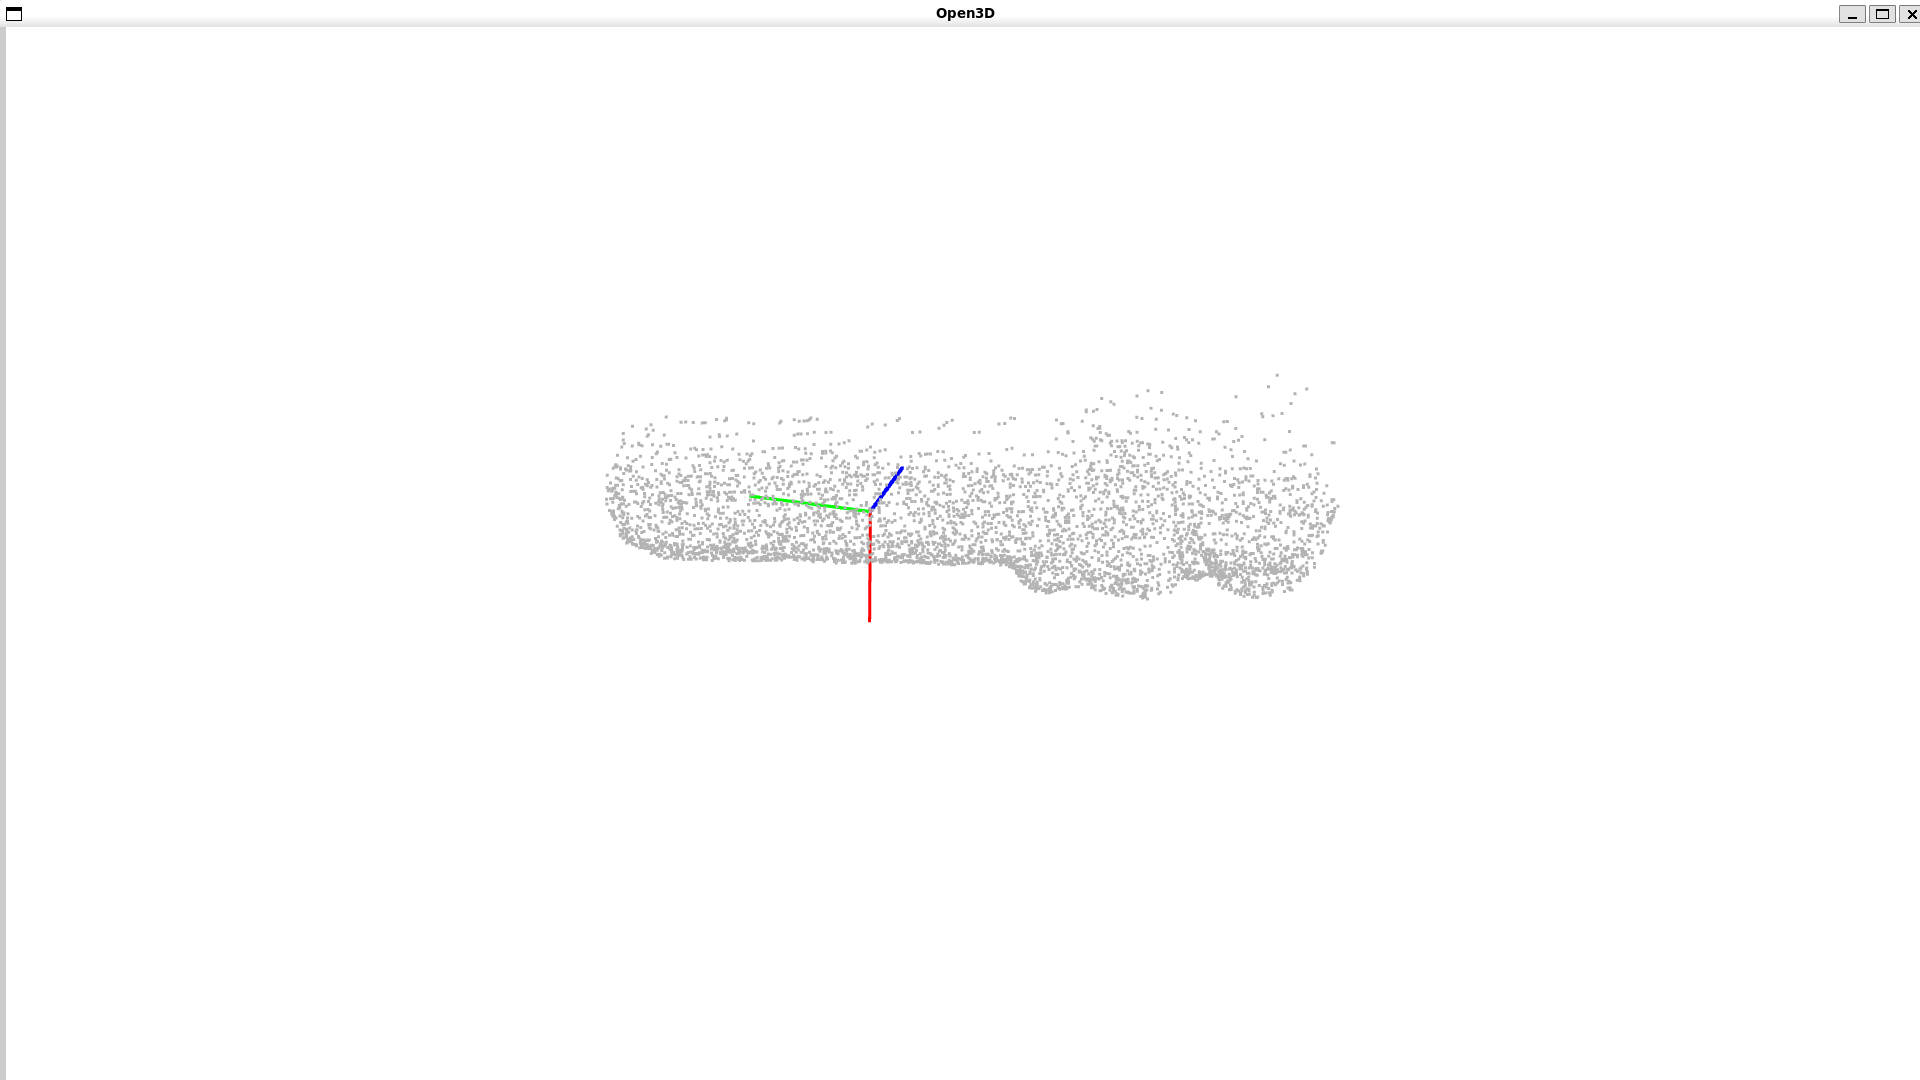
\includegraphics[width=0.95\linewidth]{F4-grasp-opp.jpg}
  \caption{Failure mode F4. Object grasped at incorrect orientation.}
  \label{fig:failure_mode_F4}
\end{figure}

\subsection{Failure Distribution by Condition}
\label{sec:failure-distribution-by-condition}

Table~\ref{tab:failure_modes} reports the failure mode distribution per condition. 

\begin{table}[htbp]
  \centering
  \caption{Failure mode counts per condition (144 trials each).}
  \label{tab:failure_modes}
  \begin{tabular}{llllll}
    \toprule
    Condition & F1 (grip) & F2 (no pose) & F3 (kinematic) & F4 (orient.) & Success \\
    \midrule
    Baseline~1 & 103 & 0 & 11 & 10 & 20 \\
    Baseline~2 & 71 & 1 & 14 & 0 & 58 \\
    Final      & 1 & 7 & 25 & 0 & 111 \\
    \bottomrule
  \end{tabular}
\end{table}

\textbf{Baseline~1 (13.9\,\%).}

F1 dominates with 103 failures (71.5\,\%): unconstrained candidate selection places grasps at object extremities remote from the centroid, producing insufficient grip force during transport.

F2 does not occur (0\,\%), because no filter is active.

F3 accounts for 11 failures (7.6\,\%), concentrated at orientations that require joint configurations near the UR10e workspace boundary.

F4 accounts for 10 failures (6.9\,\%): without an axis alignment constraint, off-axis candidates generate placement orientation errors at delivery.

\textbf{Baseline~2 (40.3\,\%).}

F1 falls from 103 to 71 (49.3\,\% of trials): centroid distance constraints concentrate candidate selection in the stable handle region, eliminating the majority of extremity grasps. Residual F1 occurs where the flat fingertip contacts the cylindrical handle surface at a marginal line-contact point insufficient to sustain grip during transport.

F2 appears at 1 trial (0.7\,\%), where point cloud degradation at the handle region causes all candidates to be rejected after centroid filtering.

F3 increases marginally from 11 to 14 (9.7\,\%): constraint-selected candidates at certain orientations require slightly harder joint configurations than the unconstrained top-ranked candidate, expanding the planning failure set.

F4 is eliminated (0\,\%): the axis projection constraint rejects candidates whose gripper axis not aligns with the object's principal axis.

\textbf{Final (77.1\,\%).}

F1 falls to 1 (0.7\,\%): the custom silicone fingertip eliminates nearly all residual grip failures. 

F2 increases from 1 to 7 (4.9\,\%): The increment reflects inter-session point cloud variability. Final condition trials were conducted in a separate experimental session in which minor object placement offsets caused transient reductions in handle-region candidate density. No algorithmic change causes this increase.

F3 increases from 14 to 25 (17.4\,\%): driven by O3 (12$\rightarrow$15) and O7 (1$\rightarrow$9). The orientation-specific F3 pattern is examined in \cref{sec:failure-distribution-by-orientation}.

F4 remains 0 (0\,\%): orientation compliance is maintained at Baseline~2 level; the fingertip modification does not interact with the axis alignment constraint.

\subsection{Failure distribution by orientation}
\label{sec:failure-distribution-by-orientation}

\begin{table}[htbp]
  \centering
  \caption{Baseline~1 orientation cluster classification (O1--O8).}
  \label{tab:baseline1_orientation_clusters}
  \begin{tabular}{lllll}
    \toprule
    Orientation & F1 & F2 & F3 & F4 \\
    \midrule
    O1 & 10 & 0 & 0 & 2 \\
    O2 & 14 & 0 & 0 & 2 \\
    O3 & 18 & 0 & 0 & 0 \\
    O4 & 14 & 0 & 0 & 0 \\
    O5 & 15 & 0 & 0 & 2 \\
    O6 & 13 & 0 & 0 & 1 \\
    O7 & 5 & 0 & 11 & 0\\
    O8 & 14 & 0 & 0 & 3 \\
    \bottomrule
  \end{tabular}
\end{table}

\begin{table}[htbp]
  \centering
  \caption{Baseline~2 orientation cluster classification (O1--O8).}
  \label{tab:baseline2_orientation_clusters}
  \begin{tabular}{lllll}
    \toprule
    Orientation & F1 & F2 & F3 & F4 \\
    \midrule
    O1 & 9 & 0 & 0 & 0 \\
    O2 & 16 & 0 & 0 & 0 \\
    O3 & 5 & 1 & 12 & 0 \\
    O4 & 2 & 0 & 0 & 0 \\
    O5 & 10 & 0 & 1 & 0 \\
    O6 & 11 & 0 & 0 & 0 \\
    O7 & 13 & 0 & 1 & 0\\
    O8 & 5 & 0 & 0 & 0 \\
    \bottomrule
  \end{tabular}
\end{table}

\begin{table}[htbp]
  \centering
  \caption{Final orientation cluster classification (O1--O8).}
  \label{tab:final_orientation_clusters}
  \begin{tabular}{lllll}
    \toprule
    Orientation & F1 & F2 & F3 & F4 \\
    \midrule
    O1 & 1 & 0 & 0 & 0 \\
    O2 & 0 & 0 & 0 & 0 \\
    O3 & 0 & 3 & 15 & 0 \\
    O4 & 0 & 2 & 1 & 0 \\
    O5 & 0 & 1 & 0 & 0 \\
    O6 & 0 & 0 & 0 & 0 \\
    O7 & 0 & 0 & 9 & 0\\
    O8 & 0 & 1 & 0 & 0 \\
    \bottomrule
  \end{tabular}
\end{table}

The 8-orientation matrix reveals structured failure patterns. Three clusters emerge from per-orientation success rate analysis in the 3 conditions.

\textbf{Epistemic uncertainty and low-confidence orientations lead to F1.}
In Baseline~2, orientations O1, O2, O5, O6, and O7 produce elevated F1 rates (9--16 failures per orientation out of 18 trials). These orientations yield few surviving candidates after centroid filtering --- typically one to two candidates, compared to five to ten at well-represented orientations. The sparse pool is consistent with high epistemic uncertainty: the vMF-Contact model has limited training coverage of these viewpoints, producing a broad, low-density distribution that generates few high-confidence candidates within the centroid zone. The system selects from a small, low-confidence pool, increasing the probability of selecting a candidate at a marginal contact position where the flat fingertip provides insufficient grip.

\textbf{F2 elevates and F1 almost eliminates in the final condition.}
In final condition, F2 failures occur at a small number of orientation cells (O3\,=\,3, O4\,=\,2, O5\,=\,1, O8\,=\,1). This may be because the hardwares were repositioned between sessions, causing minor variations in object placement and point cloud coverage. The F2 failures are concentrated at orientations where the handle region is partially occluded or where sensor noise degrades point cloud coverage, reducing the number of candidates that survive the centroid distance filter.
In all observed F2 cases, a minor object repositioning resolved the failure in a subsequent attempt. 
F2 failures are recorded as failures in the trial protocol, with no repositioning permitted between delivery and execution. In a production deployment, the environment in which the object is placed should avoid scenes with complex lighting conditions, and a lightweight position retry heuristic would recover the majority of these cases at negligible operational cost.

The custom silicon fingertip substantially resolves the F1 failures in the Final condition. The single residual F1 at O1 remains the only orientation-specific F1. This may also due to noise in the point cloud image because of the environment, affecting the centroid distance filter.


% F2 failures are recorded as failures in the trial protocol, with no repositioning permitted between delivery and execution. 
% In a production deployment, a lightweight position retry heuristic would recover the majority of these cases at negligible operational cost.

% \textbf{Normal cluster.} 
% The remaining orientations produce success rates at or above the overall Final condition rate of 77.1\,\%. 
% At these orientations, the model generates five or more centroid-filtered candidates with sufficient confidence, the top-ranked candidate lies on the handle in the stable contact zone, and the custom fingertip provides reliable grip.

\textbf{F3 dominates failure at critical orientations O3 and O7 in the final condition.}
O3 and O7 account for 24 of the 25 F3 failures in the Final condition and constitute the primary F3 cluster (\cref{tab:baseline1_orientation_clusters}--\cref{tab:final_orientation_clusters}).
%  At O3, centroid-filtered candidates lie systematically near the UR10e workspace boundary regardless of condition; the fingertip change does not affect this kinematic geometry. The elevated O7 F3 count in the Final condition (9) is more consistent with Baseline~1 (11) than with Baseline~2's atypically low rate (1), suggesting Baseline~2's O7 result reflects sampling variance across the 18 trials at that orientation.
The F3 pattern at O3 is constraint-induced rather than an intrinsic property of the kinematic envelope. In Baseline~1, unconstrained candidate selection produces kinematically accessible poses at O3: all 18 trials proceed to motion planning, but all fail through grip force insufficiency (F1\,=\,18, F3\,=\,0). Once centroid distance constraints restrict candidate selection in Baseline~2, the feasible candidate set at O3 is confined to approach angles near the UR10e workspace boundary, producing F3\,=\,12. The pattern intensifies in the Final condition (F3\,=\,15, F2\,=\,3). O3 achieves zero successes across all three conditions.

At O7, F3 rates vary across conditions (Baseline~1: 11, Baseline~2: 1, Final: 9). The anomalously low Baseline~2 rate likely reflects session-level sampling variance: centroid-constrained candidate selection at O7 happened to favour kinematically accessible poses in the Baseline~2 session, while both the Baseline~1 and Final sessions encountered workspace boundary proximity more frequently due to minor inter-session differences in object placement.

Both orientations are included in the full-matrix success rate denominator, as they represent real failure conditions in the deployment. The success rate over the six kinematically productive orientations (O1, O2, O4, O5, O6, O8), excluding O3 and O7, is \textbf{94.4\,\%} in the Final condition, compared to 77.1\,\% over the full matrix.

One practical solution to this failure mode is to avoid the critical orientations O3 and O7 in deployment, either by instructing the AGV to deliver the object in a different orientation or by rotating the object in situ before grasping. This is a simple operational mitigation that does not require any algorithmic change.

% The pre-emptive reachability filter described in Section~3.4.5 is the direct solution and is identified as future work.

Another pratical solution to this failure mode is to substitute the object axis alignment constraint at these critical orientations (O3, O7 and possibly O5) with a new reachability filter. It only limits candidates to those whose gripper axis is aligned with the object's principal axis, rather than enforcing a strict orientation. This would expand the candidate set at O3 and O7, allowing the planner to select kinematically feasible poses. But it comes with inverted placement at these orientations as a trade-off. \textbf{TODO: add link to Future Work}

% The constraint algorithm surfaces a latent kinematic boundary that unconstrained selection avoids by ranking high-confidence candidates that happen to lie in kinematically central regions of the workspace.



% The custom silicone fingertip substantially resolves this cluster: in the Final condition, F1 falls to zero at O2, O5, O6, and O7, and to a single trial at O1. The near-elimination of F1 at orientations with sparse candidate pools confirms that the dominant failure mechanism in Baseline~2 was mechanical grip insufficiency at marginal contact positions, rather than incorrect candidate ranking. The single residual F1 at O1 remains the only orientation-specific F1 in the Final condition.



\subsection{Failure distribution by position}
\label{sec:failure-distribution-by-position}

\begin{table}[htbp]
  \centering
  \caption{Baseline~1 position cluster classification (P1--P6).}
  \label{tab:baseline1_position_clusters}
  \begin{tabular}{lllll}
    \toprule
    position & F1 & F2 & F3 & F4 \\
    \midrule
    P1 & 16 & 0 & 2 & 3 \\
    P2 & 17 & 0 & 3 & 3 \\
    P3 & 16 & 0 & 3 & 1 \\
    P4 & 15 & 0 & 3 & 0 \\
    P5 & 20 & 0 & 0 & 2 \\
    P6 & 19 & 0 & 0 & 1 \\
    \bottomrule
  \end{tabular}
\end{table}

\begin{table}[htbp]
  \centering
  \caption{Baseline~2 position cluster classification (P1--P6).}
  \label{tab:baseline2_position_clusters}
  \begin{tabular}{lllll}
    \toprule
    position & F1 & F2 & F3 & F4 \\
    \midrule
    P1 & 11 & 0 & 2 & 0 \\
    P2 & 14 & 1 & 1 & 0 \\
    P3 & 12 & 0 & 3 & 0 \\
    P4 & 11 & 0 & 1 & 0 \\
    P5 & 13 & 0 & 3 & 0 \\
    P6 & 10 & 0 & 4 & 0 \\
    \bottomrule
  \end{tabular}
\end{table}

\begin{table}[htbp]
  \centering
  \caption{Final position cluster classification (P1--P6).}
  \label{tab:final_position_clusters}
  \begin{tabular}{lllll}
    \toprule
    position & F1 & F2 & F3 & F4 \\
    \midrule
    P1 & 0 & 0 & 5 & 0 \\
    P2 & 0 & 3 & 0 & 0 \\
    P3 & 0 & 0 & 5 & 0 \\
    P4 & 0 & 0 & 4 & 0 \\
    P5 & 1 & 1 & 6 & 0 \\
    P6 & 0 & 3 & 5 & 0 \\
    \bottomrule
  \end{tabular}
\end{table}

Position effects are secondary to orientation effects. 
Success rate variation across the six positions within any given orientation is small relative to the inter-orientation variation. 

\textbf{F1 and F3 show no clear pattern across positions.} 
In Baseline~1, F1 is the dominant failure mode and is distributed across all six positions (P1--P6) with no clear pattern. In Baseline~2, F1 is reduced but remains evenly distributed across positions. In the Final condition, F1 is nearly eliminated and does not show any position-specific clustering.

F3 is also mostly evenly distributed across positions. The position effect on F3 is likely a secondary consequence of the orientation effect: certain orientations produce kinematically challenging poses that are more likely to occur at specific positions due to the robot's reachability envelope.

\textbf{F2 is concentrated at P2 and P6.}
P2 and P6 have higher F2 incidence compared to other positions. (\cref{tab:final_position_clusters}). P2 and P6 are postions where the object is placed closer to the robot. This may lead to partial occlusion. reducing the number of contact candidates that survive the centroid distance filter. A minor object repositioning would resolve the failure in a subsequent attempt as described in \cref{sec:failure-distribution-by-orientation}. 

% Position has no measurable effect on F3 or on the F1 cluster pattern. 
% These cells are concentrated at specific object positions where partial occlusion or sensor noise degrades point cloud coverage at the handle region, 
\section{Summary}
\label{sec:results-summary}

Three conclusions follow from the experimental results.

First, centroid-based geometric constraints are necessary. 
Unconstrained inference (Baseline~1, 13.9\,\%) is not viable for this deployment task; 
F1 and F4 failures are systematic and frequent. The constraints raise performance to 40.3\,\% (Baseline~2), confirming that the identified failure modes are addressable through principled algorithmic modification and that the effect is large.

Second, hardware adaptation is equally necessary. Baseline~2 (40.3\,\%) does not meet the threshold for reliable industrial operation. The custom fingertip raises performance to 77.1\,\% (Final), 
demonstrating that hardware-object compatibility is a load-bearing factor independent of algorithm quality. Neither adaptation is sufficient alone; the combined system is required.

Third, the 77.1\,\% Final result demonstrates viability under conditions more demanding than the published vMF-Contact benchmark of 72.7\,\%~\cite{shi2025}, despite three systematic deployment disadvantages. The residual failure modes (F3 workspace limits, epistemic uncertainty at specific orientations, occasional F2) identify the remaining improvement levers and are examined in Chapter~5.


% ============================================================
\chapter{Discussion}
\label{chap:discussion}
% ============================================================

\section{Interpreting the Three-Condition Results}

The three-condition design produces two independent effect measurements with clear attribution. 

The Baseline~1 to Baseline~2 transition (from 13.9\,\% to 40.3\,\%) quantifies the software contribution of centroid-based constraints, with hardware held constant. The Baseline~2 to Final transition (from 40.3\,\% to 77.1\,\%) quantifies the hardware contribution of the custom fingertip, with the algorithm held constant. Both effect sizes are large and unambiguous; neither contribution is marginal.

The magnitude of the Baseline~1 result deserves emphasis. A success rate of 13.9\,\% on 144 trials means the unconstrained algorithm succeeds at this task in fewer than one in 6 attempts. Comparing with the vMF-Contact algorithm, which achieves 72.7\,\% on a controlled benchmark~\cite{shi2025}, it indicates that the base method is unusable without adaptation in this deployment context. The two centroid-based constraints address a principled omission in the original algorithm. The object-level geometric priors are necessary in this deployment context rather than compensating for incidental environmental factors.

The Baseline~2 result (40.3\,\%) identifies an equally important finding: a system that selects mechanically valid, correctly oriented candidates fails half the time, because the gripper cannot sustain grip through lift-up and transport. Algorithmic improvement is necessary but not sufficient. 
The custom fingertip addresses a hardware-object mismatch that no modification to the inference pipeline can resolve. The combined system (Final, 77.1\,\%) demonstrates that both dimensions of the deployment problem must be addressed independently.

The 77.1\,\% Final result demonstrates viability under conditions more demanding than the Shi et al.~\cite{shi2025} benchmark along three independently measurable axes: lower grip force (125\,N versus 235\,N), a heavier object ($\sim$2\,kg versus $\sim$1\,kg), and a stricter success criterion encompassing the full pick-transport-place sequence. The benchmark conditions are more favourable along every axis. That the deployment result maintains performance above the benchmark rate under these compounding disadvantages confirms that the specific adaptations are sufficient to sustain performance despite the deployment handicap. 

This is not a claim that the adapted system is intrinsically superior to the base algorithm on diverse objects under controlled conditions. It is rather evidence that the adaptations are correctly targeted at the specific factors that would otherwise suppress performance below the benchmark in this deployment context.

\section{Failure Mode Analysis: Causes and Implications}
\label{sec:failure-mode-analysis-discussion}

Understanding the causes of residual failures in the Final condition is more useful for guiding future work than the top-line success rate.

\textbf{Epistemic uncertainty and the low-confidence orientation cluster.} 
The orientation-dependent F1 cluster identified in \cref{sec:failure-distribution-by-orientation} reflects the epistemic uncertainty property of the vMF-Contact model discussed in \textbf{TODO: should be a specific section of chapter 2}. At orientations underrepresented in the training distribution, the model produces a broad, low-density vMF distribution: few contact candidates fall within the centroid zone, and those that do carry low model confidence. 
The system selects the highest-ranked surviving candidate, but this candidate is disproportionately likely to fall at the boundary of the mechanically stable grip zone, where the flat fingertip provides insufficient friction to hold a 2\,kg object through a full transport trajectory.

The failure sequence --- high epistemic uncertainty $\rightarrow$ sparse centroid-filtered candidates $\rightarrow$ boundary contact selection $\rightarrow$ F1 --- validates the theoretical motivation for probabilistic uncertainty modelling introduced in Chapter~2. 

It also identifies the appropriate intervention. 
(1) A custom designed silicon fingertip which is introduced in \cref{sec:custom-fingertip-design} and implemented in final condition shows substantial improvement in grasp performance. 
(2) Alternatively, orientation pre-screening at delivery time, biasing AGV placement toward orientations with known high coverage, would reduce exposure to the low-confidence cluster without any algorithm modification.

\textbf{Positional sensitivity.} 
F2 failures are few, position-sensitive, and operationally recoverable. 
In all observed cases, a minor repositioning of the object resolved the failure in a subsequent attempt. 
A position retry heuristic in the delivery placement protocol, or a feedback signal from the inference node to the AGV controller, would address the majority of F2 cases at negligible cost.

\textbf{Kinematic infeasibility.} 
F3 failures at specific orientations reflect the UR10e workspace boundary, not algorithm or hardware behaviour. The appropriate solution is a pre-execution reachability check that aligns the grip axis with the object principal axis (in both directions) before final selection. Integrating and validating this filter on the current trial matrix is the most direct path to reducing F3 failures and improving the full-matrix success rate beyond 77.1\,\%. A prototype implementation of reachability filter is introduced in the \textbf{TODO: Appendix}. 

\section{Deployment Evaluation as a Research Contribution}

The structured deployment evaluation contributes methodologically, independently of the algorithm and hardware adaptations. The three-condition design --- 432 trials, two isolated factorial comparisons, failure mode stratification across a position $\times$ orientation matrix --- illustrates how the gap between laboratory benchmark performance and real industrial deployment can be characterised and decomposed.

The existing evaluation paradigm for grasping methods reports isolated grasp success under controlled conditions: calibrated placement, clean point clouds, success measured at gripper closure. This protocol is well-suited for comparing methods under reproducible conditions; 
it is not designed to characterise deployment performance. Deployment success is a system-level property. It compounds hardware-object compatibility, sensor noise from real environments, kinematic constraints of the specific robot platform, and downstream task requirements. None of these factors appears in isolated grasp benchmarks. The gap between 72.7\,\% (benchmark) and 13.9\,\% (this deployment without adaptation) is the compound product of missing geometric priors, hardware-object force mismatch, and a stricter success criterion operating together.

The Baseline~1 result demonstrates that published benchmark performance does not transfer to a real deployment without adaptation. Baseline~2 and Final progressively close the gap by addressing one factor at a time, with each addressed factor producing a large, measurable improvement. It systematically decomposites the benchmark-to-deployment gap into independently attributable factors, which constitutes one structured case study in how learning-based grasping methods require characterisation before industrial deployment, as a complement to, rather than a replacement for, laboratory benchmarks. Establishing whether this evaluation template generalises across object classes, gripper types, and deployment contexts is itself a direction for future work. The present study provides a single, carefully executed case study rather than a general methodology.

\section{Limitations}
\label{sec:limitations}

\textbf{Object-specificity of centroid parameters.} The centroid distance thresholds (\param{grasp\_cog\_max\_dist\_th} = 0.025\,m, \param{grasp\_cog\_min\_dist\_th} = 0.01\,m) and axis projection tolerance are calibrated to the angle grinder's geometry. Extending the system to a second class requires repeating the parameter validation procedure. Whether a unified parameter set generalises across a family of elongated asymmetric objects remains an open question.

\textbf{Single-object scene requirement.} The centroid proxy is computed from the full filtered point cloud without instance segmentation. In a multi-object scene, the computed centroid averages across all objects present, making the spatial filter geometrically undefined. The system therefore requires single-object placement in the delivery zone. This is a constraint of the CoG approach, not of vMF-Contact itself; the base algorithm handles cluttered multi-object scenes through contact-normal sampling. Introducing an instance segmentation module --- a PointNet++~\cite{qi2017pointnet2} segmentation head or a dedicated 3D instance segmentation network --- would restore multi-object capability while preserving the CoG constraint logic, and is the most direct path to extending the current system to cluttered scenes.

\textbf{Residual F3 failures.} The F3 failure cluster at specific orientations is unaddressed in the current experimental system. These failures are primarily a function of the UR10e workspace geometry and the constraint-selected candidate set; F3 rates rise across conditions as constraints progressively restrict candidate selection toward workspace-boundary poses. The pre-emptive reachability filter (Section~3.4.5) is the appropriate solution and has been applied on a small set of experiemnts. It will be introduced in \textbf{TODO: Appendix}

% but was not validated in time for the reported trials. Until integrated, the system's reliable operating envelope excludes the F3 cluster orientations, even though they are correctly included in the full-matrix success rate.

\textbf{Model coverage at specific orientations.} The epistemic uncertainty cluster identifies orientations at which the vMF-Contact model has limited training coverage of the angle grinder. This cannot be resolved through the constraint modifications alone. Additional training data at underrepresented viewpoints, or a confidence-weighted selection policy, would address the residual F1 failures in this cluster.

\textbf{Gripper selection trade-off.} The Robotiq 2F-140 was chosen for geometric compatibility with the angle grinder handle at the cost of a 47\,\% reduction in grip force relative to the 2F-85 (125\,N versus 235\,N). The custom fingertip partially compensates for this, but does not restore grip force to 2F-85 levels. A gripper offering both wide jaw opening and higher force would likely improve performance further while preserving geometric compatibility.

\section{Deployment Recommendations}
\label{sec:deployment-recommendations}

The results and limitations define a specific operating envelope. The current system is suited to some industrial contexts and not others, and the boundary between them follows directly from the failure mode analysis.

\textbf{Suitable contexts.} The system is well-matched to circular factory return streams: single objects of a known class delivered by AGV at variable position and orientation, moderate throughput compatible with a 3--5\,second pipeline latency, and an operational tolerance for a 77.1\,\% first-attempt success rate with a retry path for failed attempts. In the current cell, F1 failures (object dropped mid-trajectory) are detected via visual inspection. F2 and F3 failures are reported by the inference and planning nodes respectively. This detection infrastructure is a prerequisite for any retry loop. Deployments without it cannot safely implement automated retry. The broader class of circular manufacturing scenarios shares the cell's operating properties and fits the system's envelope for the same reasons.

\textbf{Unsuitable contexts.} High-takt automated assembly lines are outside the current operating envelope: the inference-and-planning latency is incompatible with short cycle times, and a single F3 or F1 failure interrupts the line. Multi-object cluttered scenes require an instance segmentation module before the CoG constraints become applicable. Safety-critical applications requiring reliability above 95\,\% would need the F3 reachability filter, epistemic uncertainty mitigation, and additional validation before deployment. Novel object geometries require re-parameterisation of the CoG thresholds and fingertip contact validation because the current parameters are specific to the angle grinder and should not be applied to other object classes without verification.

Each unsuitability is addressable through specific, tractable future work. None is intrinsic to the approach. The system is a validated starting point for industrial learning-based grasping; closing the remaining performance gaps is a matter of engineering effort rather than fundamental research.


% ============================================================
\chapter{Conclusion}
\label{chap:conclusion}
% ============================================================

\section{Summary}
\label{sec:conclusion-summary}

This thesis asked: to what extent can the pick-and-place with unconstrained vMF-Contact algorithm work in a real production scenario? What other constraints can be applied to improve the grasping success rate of an angle grinder compared to unconstrained vMF-Contact inference?

The answer is unambiguous. 
Unconstrained vMF-Contact inference achieves a success rate of 13.9\,\% on the $3 \times 8 \times 6$ trial matrix. Centroid-based constraints raise this to 40.3\,\%. The addition of a custom curved silicone fingertip raises it further to 77.1\,\%. The improvement from constraints alone (approximately 26.4 percentage points) demonstrates that the algorithmic adaptation is both necessary and effective. 
The further improvement from the fingertip (approximately 36.8 percentage points) demonstrates that hardware-object compatibility is an independent, load-bearing factor that no algorithm modification can substitute for.

Three contributions realise these results. 

Contribution~A introduces two parameter-governed centroid-based constraints into the vMF-Contact inference pipeline: an annular grip zone defined relative to the object's geometric centroid proxy, and a gripper-axis alignment constraint with the object's principal axis. These address grip force insufficiency and orientation error --- the two dominant failure modes of unconstrained inference on this task --- through principled geometric constraints rather than post-hoc filtering.

Contribution~B is a custom fingertip for the Robotiq 2F-140, incorporating a curved contact surface matched to the angle grinder handle and a silicone friction layer, which addresses the grip force insufficiency that persists after algorithmic correction. 
 
Contribution~C is the ROS2 and Docker integration pipeline that enables reproducible deployment of the full system on the UR10e cell.

Contribution~D is the structured deployment evaluation, which isolates the effects of algorithmic and hardware adaptation, stratifies failure modes by orientation and position, and identifies residual failure clusters for future work. The evaluation demonstrates that the gap between benchmark and deployment is structured and closeable, not random and irreducible.

The Final condition result of 77.1\,\% demonstrates viability under conditions more demanding than the published vMF-Contact benchmark of 72.7\,\%~\cite{shi2025}, with lower grip force, a heavier object, and a stricter success criterion, confirming that the targeted adaptations are sufficient to maintain above-benchmark performance despite the deployment disadvantage. Both hardware and software adaptations are necessary.

\section{Research Gaps Addressed}

\textbf{Gap A --- Missing geometric priors.} Prior learning-based grasping methods, including vMF-Contact, encode local contact geometry but not object-level spatial relationships. The centroid-based constraints introduced in Contribution~A directly address this omission. The Baseline~1 to Baseline~2 result provides quantitative evidence that these priors are necessary for this task class: without them, the algorithm fails on nearly every trial.

\textbf{Gap B --- Absence of systematic deployment evaluation.} Prior work provides benchmark comparisons but not structured deployment studies with failure mode stratification, real hardware-object constraints, and a full pick-transport-place success criterion. The 432-trial evaluation across three conditions, eight orientations, and six positions fills this gap for the specific deployment studied here. The failure mode analysis demonstrates what this style of evaluation reveals that isolated benchmarks do not: the specific conditions under which a validated method succeeds and fails in a real industrial cell.

\section{Future Work}

Four directions follow directly from the limitations identified in \cref{sec:limitations}.

\textbf{Kinematic reachability filter.} F3 failures at specific orientations are the most directly addressable residual failure mode. A prototype reachability filter that evaluates kinematic feasibility before candidate selection is implemented in \textbf{TODO: Appendix}. Integrating and validating this filter on the current trial matrix is the most immediate path to improving the full-matrix success rate beyond 77.1\,\%, without changes to the algorithm or hardware.

% \textbf{Confidence-weighted candidate selection.} The epistemic uncertainty failure cluster --- orientations at which the model generates few low-confidence candidates, producing elevated F1 rates --- is addressable through a selection policy that penalises low-confidence candidates even when they satisfy the spatial filters. A confidence threshold on surviving candidates, or an explicit preference for candidates with probability mass above a learned coverage threshold, would reduce the probability of selecting marginal contact positions at underrepresented orientations.

\textbf{Instance segmentation for multi-object scenes.} The current system requires single-object placement because the centroid proxy is computed from the full point cloud. Adding an instance segmentation module --- a PointNet++~\cite{qi2017pointnet2} segmentation head or a dedicated 3D network --- would restore the ability to handle cluttered multi-object scenes while preserving the CoG constraint logic. This is the primary architectural extension required to broaden the system's applicability beyond single-object delivery zones.

\textbf{Parameter generalisation.} The centroid distance and axis projection thresholds are calibrated to the angle grinder's geometry. Validating whether a common parameter set applies across a family of elongated asymmetric objects, or deriving the thresholds analytically from measurable object properties (handle length, centroid offset, gripper jaw width), would reduce the per-class calibration overhead and extend the system's practical range.

\section{Closing}
\label{sec:closing}

Learning-based grasping methods achieve strong benchmark performance. The central finding of this thesis is an answer to why industrial deployment consistently falls short: algorithms encode no object-level geometric priors, hardware-object compatibility is absent from evaluation protocols, and benchmark success criteria measure a narrow proxy for the system-level outcome that deployment requires.

The adaptations introduced here, including centroid-based constraints and a purpose-designed fingertip, are not patches on a broken method. They are the minimum necessary engineering to connect a laboratory-validated algorithm to a specific deployment context. That connection required understanding what the algorithm could not do, why the hardware was insufficient, and how to measure both in a way that separates their contributions. The result where 77.1\,\% success on a task the base algorithm failed at 13.9\,\% is evidence that the gap between benchmark and deployment is structured and closeable. Closing it systematically, across object classes and deployment contexts, is the work that remains.


% ============================================================
% BIBLIOGRAPHY
% ============================================================
\bibliographystyle{IEEEtran}
\bibliography{references}

% ============================================================
% APPENDIX
% ============================================================
\appendix

\chapter{Kinematic Reachability Filter}
\label{chap:appendix-reachability}

\section{Motivation}
\label{sec:appendix-motivation}

In the Final condition (Section~4.3), kinematic infeasibility (F3) is the dominant residual failure mode: 25 of 144 trials (17.4\,\%) end in motion-planner failure. Two orientations account for 96\,\% of these failures: O3 (15 of 18 trials) and O7 (9 of 18 trials). O3 achieves zero successes across all three experimental conditions.

% The F3 pattern is constraint-induced rather than intrinsic to the robot's workspace. In Baseline~1, unconstrained vMF-Contact inference selects kinematically accessible candidates at O3 and O7 — all 18 O3 trials reach the motion planner, but all fail through grip force insufficiency (F1\,=\,18, F3\,=\,0). The centroid distance constraints introduced in Contribution~A confine candidate selection to the handle region, but handle-region candidates at O3 and O7 systematically require approach angles near the UR10e workspace boundary. The motion planner then fails to find collision-free joint trajectories, producing F3 failures.

Two operational mitigations were identified in Section~5.2: restricting AGV delivery to orientations outside the F3 cluster, or adding a pre-execution reachability check that filters candidates with approach geometries unlikely to be kinematically feasible before the motion planner is invoked. This appendix describes the second approach, implemented and evaluated after the main controlled experiment reported in Chapter~4.

\section{Filter Design}
\label{sec:appendix-filter-design}
The reachability filter extends the existing constraints set of \cref{sec:vmf-contact-inference} with two additional directional constraints on the grasp approach geometry. Both checks are geometric heuristics — lightweight vector operations computed from the candidate pose — that pre-discard approach directions associated with workspace-boundary configurations without invoking the IK solver or motion planner.

\paragraph{Filter B1 — Frontal projection constraint.}

\begin{figure}
  \centering
  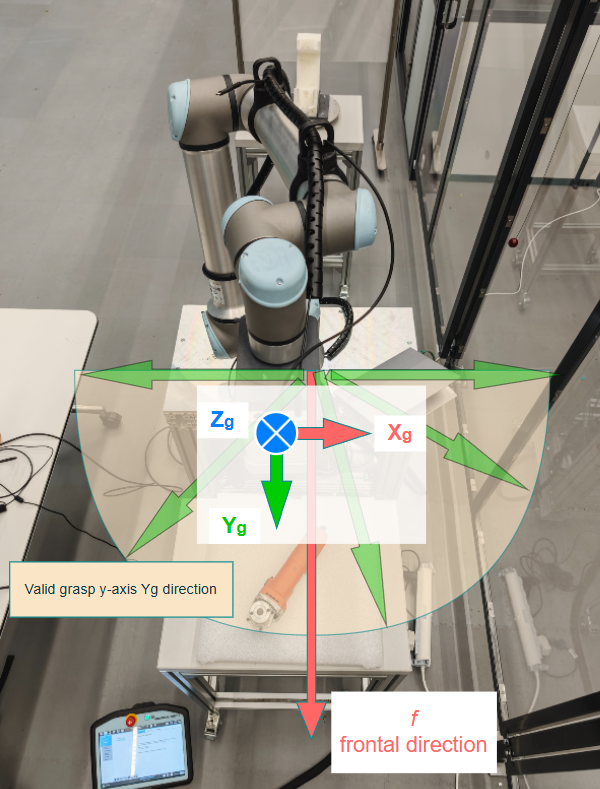
\includegraphics[width=0.95\linewidth]{frontal-overview-1.png}
  \caption{This figure shows the actual spatial representation of the frontal projection constraint. The gripper y-axis \param{y\ensuremath{\sb{g}}} should be facing the robot's frontal direction $\mathbf{f}$.}
  \label{fig:frontal-overview}
\end{figure}

\begin{figure}
  \centering
  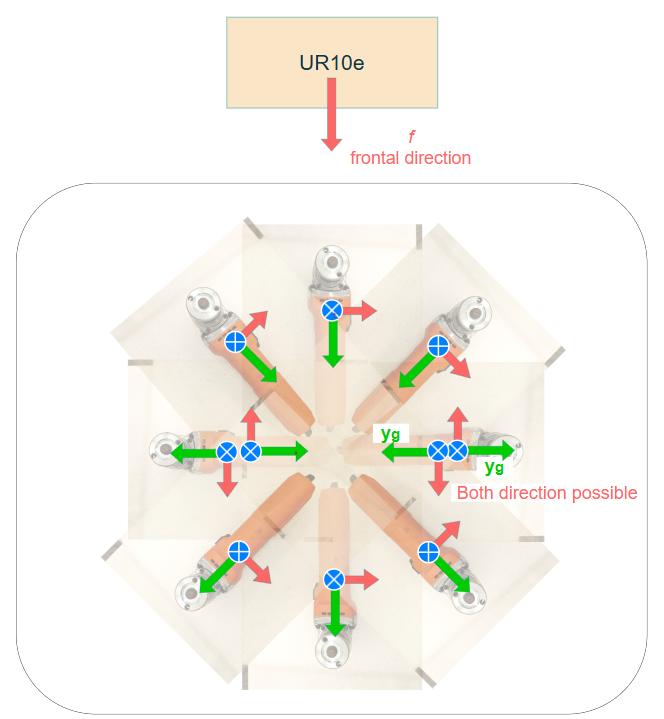
\includegraphics[width=0.95\linewidth]{frontal-orient.png}
  \caption{A representation of the possible object orientations and the gripper \param{y\ensuremath{\sb{g}}} axis after applying the frontal projection constraint.}
  \label{fig:frontal-orient-grasp}
\end{figure}

The UR10e's nominal frontal direction is defined as $\mathbf{f} = [-1,\,0,\,0]^{\!\top}$ in the world frame. For each surviving candidate, the projection of the gripper closing axis \param{y\ensuremath{\sb{g}}} onto $\mathbf{f}$ is computed:
\begin{equation}
  p = \param{y\ensuremath{\sb{g}}} \cdot \mathbf{f}.
\label{eq:frontal-projection}
\end{equation}
Candidates with $p \leq \param{grasp\_axis\_projection\_th} = 0$ are discarded. The threshold of zero requires a strictly positive projection, ensuring the gripper faces into the robot's primary workspace. Grasps directed away from the robot require shoulder and elbow joints to approach their limits in order to reach the target pose and is hense rejected. As shown in \cref{fig:frontal-overview}.

A figure that represents the possible grasp poses after applying this filter is shown in \cref{fig:vertical-grasp}. Note that there may be 2 possible grasp orientations at the two horizontal inital orientations, as their gripper y-axis \param{y\ensuremath{\sb{g}}} may either has a positive projection to the frontal axis $\mathbf{f}$, or not.


\paragraph{Filter B2 — Vertical approach constraint.}

\begin{figure}
  \centering
  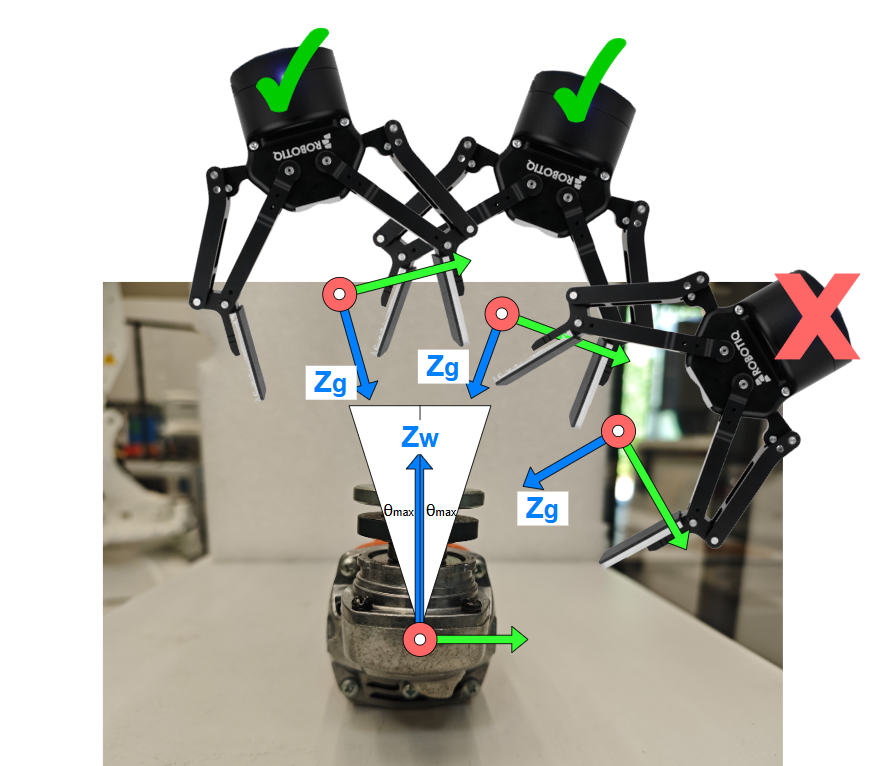
\includegraphics[width=0.95\linewidth]{vertical-grasp.png}
  \caption{This figure shows valid grasp pose after applying the filter B2-vertical approach constraint. The gripper's approach axis \param{z\ensuremath{\sb{g}}} (the z-axis of the gripper frame) is constrained to remain within $\theta_{\max}$ of the world z-axis $\param{z\ensuremath{\sb{w}}}$:}
  \label{fig:vertical-grasp}
\end{figure}

The gripper's approach axis \param{z\ensuremath{\sb{g}}} (the z-axis of the gripper frame) is constrained to remain within $\theta_{\max}$ of the world z-axis $-\param{z\ensuremath{\sb{w}}}$:
\begin{equation}
  \angle\!\left(\param{z\ensuremath{\sb{g}}}\,-\param{z\ensuremath{\sb{w}}}\right) \;\leq\; \theta_{\max}.
\label{eq:vertical-approach}
\end{equation}
The threshold $\param{grasp\_z\_negative\_world\_z\_angle\_th} = 10^{\circ}$ is applied. Candidates exceeding this angle are discarded.

% A near-vertical approach minimises wrist rotation demand and keeps the end-effector in the region of the UR10e workspace where the redundancy resolver reliably produces joint-limit-safe configurations. At O3 and O7, handle-region candidates after centroid filtering tend to have tilted approach vectors because the object's handle faces directions that require non-vertical gripper entry at those orientations; the vertical constraint pre-filters these candidates before the motion planner is invoked.

A near-vertical approach minimises wrist rotation possibility and keeps the end-effector in the region of proper grasp workspace where the gripper would not approach the object from the side. This helps avoid tilted approach and eventually manual adjustment after placement because of the object face direction. 
\section{Pipeline Integration}
\label{sec:appendix-pipeline}

Filters~B1 and~B2 are inserted beside the existing Filter A (axis alignment, \cref{sec:axis-alignment-constraint}) and before motion planning, forming a multi-stage cascade. A detailed diagram is shown in \cref{fig:filter-cascade}.

\begin{figure}
  \centering
  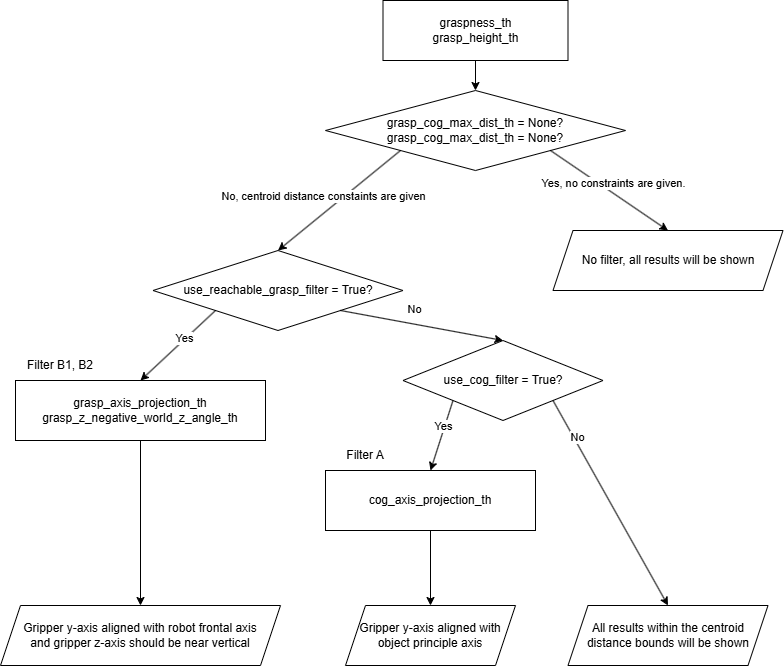
\includegraphics[width=0.95\linewidth]{filter-cascade-diagram.png}
  \caption{Multi-stage candidate filtering cascade. Filters~B1 and~B2 are pre-emptive reachability checks that discard candidates with approach geometries likely to be kinematically infeasible.}
  \label{fig:filter-cascade}
\end{figure}

Both new filters are vector arithmetic with negligible runtime cost. The pipeline latency increase relative to the Final condition is below 1\,ms per inference call. 

% The implementation is in branch \texttt{dev\_3} of the vMF-Contact fork:
% \begin{center}
% \small\url{https://github.com/YiminHu26/vMF-Contact/blob/dev_3/vmf_contact_main/test_11_save_logs.py}
% \end{center}
% (function call at lines~775--778, parameter \texttt{use\_reachable\_grasp\_filter = True}).

\section{Experimental Protocol}
\label{sec:appendix-protocol}

The evaluation uses a reduced factorial matrix: 8 object orientations (O1--O8) $\times$ 1 delivery position $\times$ 3 repetitions per cell, yielding 24 trials in total. The hardware and software configuration matches the Final condition: centroid-based constraints active (\param{grasp\_cog\_max\_dist\_th}\,=\,0.025\,m, \param{grasp\_cog\_min\_dist\_th}\,=\,0.01\,m, \param{cog\_axis\_projection\_th}\,=\,0.5), custom curved silicone fingertips, UR10e + Orbbec Femto Mega + Robotiq 2F-140. The success criterion follows \cref{sec:success-criterion} (full pick-transport-place completion without object drop) and is extended with a placement-quality sub-category, and counted as completed trials in the Success column: \textbf{PS} flags trials where the object is placed inverted relative to the intended target pose. Section~\ref{sec:appendix-ps-tradeoff} discusses the tradeoff this category reflect.

The reduced matrix isolates orientation effects at a single position. Per-orientation results are directly comparable to the Final condition per-orientation counts in \cref{tab:appendix-results} at the evaluated position, isolating the effect of the reachability filter from position-level variation.

\section{Results}
\label{sec:appendix-results}

\begin{table}[htbp]
  \centering
  \caption{Reachability filter evaluation: per-orientation failure counts and success (8\,orientations $\times$ 1\,position $\times$ 3\,trials\,=\,24\,trials total).}
  \label{tab:appendix-results}
  \begin{tabular}{lrrrrr}
    \toprule
    Orient. & F1(grip) & F2(no pose) & F3(kin.) & PS(Inverted orient.) & Success \\
    \midrule
    O1 & 0 & 0 & 0 & 2 & 3 \\
    O2 & 0 & 0 & 0 & 2 & 3 \\
    O3 & 0 & 0 & 0 & 3 & 3 \\
    O4 & 0 & 0 & 0 & 0 & 3 \\
    O5 & 0 & 0 & 0 & 3 & 3 \\
    O6 & 0 & 0 & 0 & 0 & 3 \\
    O7 & 0 & 0 & 0 & 3 & 3 \\
    O8 & 0 & 0 & 0 & 0 & 3 \\
    \midrule
    \textbf{Total} & 0 & 0 & 0 & 13 & \textbf{24 / 24} \\
    \bottomrule
  \end{tabular}
\end{table}

\cref{tab:appendix-results} summarises the overall grasping results for the new 24 trials. It delievered 100\,\% success across all orientations, with no F1, F2, or F3 failures. The residual placement defect (PS) is discussed in Section~\ref{sec:appendix-ps-tradeoff}.

\section{Analysis}
\label{sec:appendix-analysis}

\subsection{Elimination of F1, F2, and F3}
\label{sec:appendix-f1f3}

Across all 24 trials, F1, F2, and F3 are fully eliminated (Table~\ref{tab:appendix-results}), including at O3 and O7, which achieved zero and low successes respectively across all three conditions in the main experiment (\cref{sec:failure-distribution-by-orientation}).

The Fontal projection constraint (Filter B1) filters candidates whose gripper y-axis poses to the frontal direction of the robot station, which is the direct mechanism for the F3 elimination at these two orientations. Unlike the anticipated risk that a tighter candidate set at O3 and O7 would convert F3 trials into F2 trials, no F2 failures occur anywhere in the reduced matrix: the surviving candidate sets at every orientation retained at least one candidate that satisfied both new filters.  The vertical approach constraint (Filter B2, $\theta_{\max} = 10^{\circ}$) removes tilted gripper approach direction candidates before the motion planner is invoked.

The two filters also leave F1 unaffected, consistent with the two filters acting on approach geometry rather than on centroid-zone membership or axis alignment.

\subsection{Placement tradeoff of the frontal projection constraint}
\label{sec:appendix-ps-tradeoff}

Eliminating F1--F3 does not come without cost. Of the 24 trials, 13 are placed inverted relative to the intended target pose (\textbf{PS}); only O4, O6 and O8 are entirely free of a placement defect. O3, O5, and O7 are inverted in all three trials.

This is a direct tradeoff of the frontal projection constraint (Filter B1, Eq.~\eqref{eq:frontal-projection}). Filter B1 selects candidates whose gripper y-axis projects positively onto the robot's frontal direction $\mathbf{f}$, without reference to which end of the object's principal axis the candidate sits on. At orientations where the axis-alignment filter (Filter A) leaves viable candidates on both ends of the principal axis, Filter B1 can select the end that satisfies the reachability heuristic rather than the end consistent with the fixed placement target. Because the placement stage executes a single hardcoded target pose regardless of which end of the object was grasped, a candidate selected from the "wrong" end arrives inverted at the delivery position. Since the reversed placement does not have a corresponding placement target pose, in some cases the object must be manually reoriented after placement to be usable.

This tradeoff is acceptable for the current implementation. No trial drops the object, fails to reach a valid pose, or exceeds the robot's kinematic limits ($\text{F1} = \text{F2} = \text{F3} = 0$); the residual defect is confined to placement orientation, is immediately visible upon placement, and is acceptable for subsequent CT inspections. Exchanging a hard failure (F3, requiring a full retry cycle) for an immediately observable placement defect is a net improvement in a supervised deployment setting, even though it introduces a correction burden that Filters B1 and B2 alone do not remove.

\subsection{Limitations}
\label{sec:appendix-limitations}

The two new filters are geometric heuristics, not exact kinematic feasibility checks. A candidate that passes both filters is not guaranteed to be reachable; a candidate that fails one filter may in some cases be reachable via an alternative IK solution. The $10^{\circ}$ threshold for the vertical approach constraint was set empirically based on observation of F3 failure poses and has not been optimised over a parameter grid. A threshold that is too tight increases F2; one that is too loose provides insufficient F3 reduction. The precise operating range of the threshold is an open question for future work.

The reachability filter was evaluated at a single position. Although it has been discussed in \cref{sec:failure-distribution-by-position} that in previous experiments the failures show no position-specific clustering, it is based on the filter A. Position-dependent effects on the filter's performance — arising from the object's absolute location relative to the robot base frame — are not characterised in this evaluation and remain a direction for further investigation.

The placement stage itself is a further limitation exposed by this evaluation: it applies a single hardcoded target pose irrespective of grasp geometry, with no mechanism to detect whether the object was grasped along the principal axis in the orientation assumed by that target pose or the reverse. Removing PS therefore does not require reverting Filters B1 and B2; it requires an adaptive placement stage that determines, from the grasp candidate's pose relative to the object's principal axis, whether the object is being presented in the assumed orientation or reversed, and adjusts the release pose accordingly. Such a placement-detection algorithm is left for future work; the present evaluation reports the resulting PS counts explicitly rather than folding them into the Success count.

\end{document}
